\chapter{Parameteruntersuchung}
\label{chap:parameteruntersuchung}

\section{Einleitung und Vorgehensweise}
\label{sec:einleitung_und_vorgehensweise}
Grundlegend kann die Parameteruntersuchung wie eine Art Entscheidungsbaum aufgefasst werden. Dabei führt jede Entscheidung im Baum zu einer neuen Untersuchung und zu neuen Erkenntnissen. Im Verlaufe dieser Untersuchung werden somit Konzepte, Flugzustände, Komponenten und Konstellationen ausgewählt und intensiver betrachtet. Den Beginn zeichnet die grundlegende Frage aus, welches Fluggerätekonzept, i.e. Flächenflugzeug oder Multicopter, sich für einen effizienten Aufstieg in die untere Stratosphäre als optimaler erweist. \\
In der folgenden Parameteruntersuchung sei nochmal auf den Aufbau der Leistungsberechnung verwiesen, der dem eines realen Systems in umgekehrter Weise gegenübersteht (Kap. \ref{sec:leistungsberechnung}).

\section{Multicopter im Vergleich zu einem Flächenflugzeug}
\label{sec:multicopter_vs_flaechenflugzeug}
Jedes Luftfahrzeugkonzept entzieht sich einem direkten Vergleich mit einem Luftfahrzeug einer anderen Art. So weist jedes Fluggerät in seiner Gattung spezifische Vorteile auf wie der Start auf der Stelle und das Hovern in der Luft für Multicopter oder der Gleitflug für Flächenflugzeuge. Die optimale Auslegung beider führt zu unterschiedlichen Designs was die Propeller, die Motorleistung und -gewicht, Größe, Gesamtgewicht etc. betrifft. Aus diesem Grund müssen Kriterien für eine Vergleichbarkeit vorgeschrieben werden. Hierfür wird das Design des Multicopters auf das aus \cite{Anderson.2018} festgelegt, welches genauer in Kapitel \ref{sec:komponenten} beschrieben ist. Da die Flugleistungen von \cite{Anderson.2018} bekannt sind und der Quadrocopter durchaus schon im Rahmen der Anforderungen für diese Mission als optimiert betrachtet werden kann, bedarf es lediglich einer Untersuchung des Flächenflugzeuges. Dazu wird das Flächenflugzeug auf Parameter fixiert, mit denen es bereits sehr hoch aufsteigen kann. Zur Untersuchung und Vergleichbarkeit werden beide Gesamtmassen gleichgesetzt \ensuremath{m_{ges,Quadrocopter} = m_{ges,Flächenflugzeug}}. Dabei setzt sich die Masse der Flächenflugzeugbatterie   
\begin{equation}
	m_{Bat,Fl} = m_{Bat,Quad} + (m_{Mot,Quad}\cdot n_{Prop,Quad} - m_{Mot,Fl}\cdot n_{Prop,Fl}) - (1-f_P)\cdot m_{Quad}  
\end{equation}
in Bezug auf bereits gewählte Massen und auf den Quadrocopter zusammen. Der Faktor \ensuremath{f_P} kann als Penaltyfaktor verstanden werden. Dieser verringert zusätzlich die Batteriemasse, wenn das Strukturgewicht des Flächenflugzeugs das des Quadrocopters überschreitet
\begin{equation}
	f_P = \frac{m_{Flächenflugzeug}}{m_{Quad}}.
\end{equation} 
Für erste Untersuchungen wird der Penaltyfaktor auf 1 gesetzt. Dies entspricht einer sehr optimistischen Einschätzung. Im Anschluss werden die Parameter in näherer Umgebung der ersten festgesetzten Werte variiert. Dadurch kann der Einfluss auf das Leistungsverhalten und die Richtung der Optimierung bestimmt werden. Diese erste, einfache Untersuchung ist nur eine sehr oberflächliche, weil jeder Parameter nur einzeln untersucht wird. Jegliche Kombinationen von Einflüssen wie der Einfluss des Masse auf die Steiggeschwindigkeit oder vergleichbare Beziehungen werden vernachlässigt. Im Hinblick auf diese erste, kleine Optimierung ist der Kostenfaktor die maximal erreichbare Höhe beider Fluggeräte. Je nachdem welches der beiden Fluggeräte effektiver und effizienter eine maximale Flughöhe erreicht, wird es weiter untersucht und anschließend optimiert. 


\subsection{Erste Untersuchung}
\label{subsec:erste_untersuchung}
In der folgenden Tabelle sind wichtige Parameter der Ausgangskonstellation für das Flächenflugzeuges aufgelistet.
\todo[inline]{check die Einheit vom KV Wert}
\begin{center}
	\captionof{table}{wichtige Parameter des Flächenflugzeugs}
	\begin{tabular}{l l l} \hline
		Parameter & Variablenname & Wert \\ \hline
		Motormasse \ensuremath{m_{Mot}}& \texttt{m\_Mot} & \SI{106}{g} \\
		Geschwindigkeitskonstante \ensuremath{K_V} & \texttt{K\_V} & \SI{1390}{RPM/V} \\
		maximaler Dauerstrom \ensuremath{I_{max}} & \texttt{I\_max} & \SI{25}{A} \\
		Propeller & \texttt{prop\_name} & 9x7 \\
		Anzahl Propeller \ensuremath{n_{Prop}} & \texttt{n\_prop} & \SI{1}{} \\
		Auslegungsgleitzahl \ensuremath{E^{\star}} & \texttt{E\_stern} & \SI{4}{} \\
		Auslegungsgeschwindigkeit \ensuremath{V^{\star}} & \texttt{V\_stern} & \SI{100}{km/h} \\
		Gleitzahl \ensuremath{E} & \texttt{E} & \SI{4}{} \\ \hline
	\end{tabular}	
	\label{tab:flzg_parameter}
\end{center}

\begin{figure}[H]
%\centering
	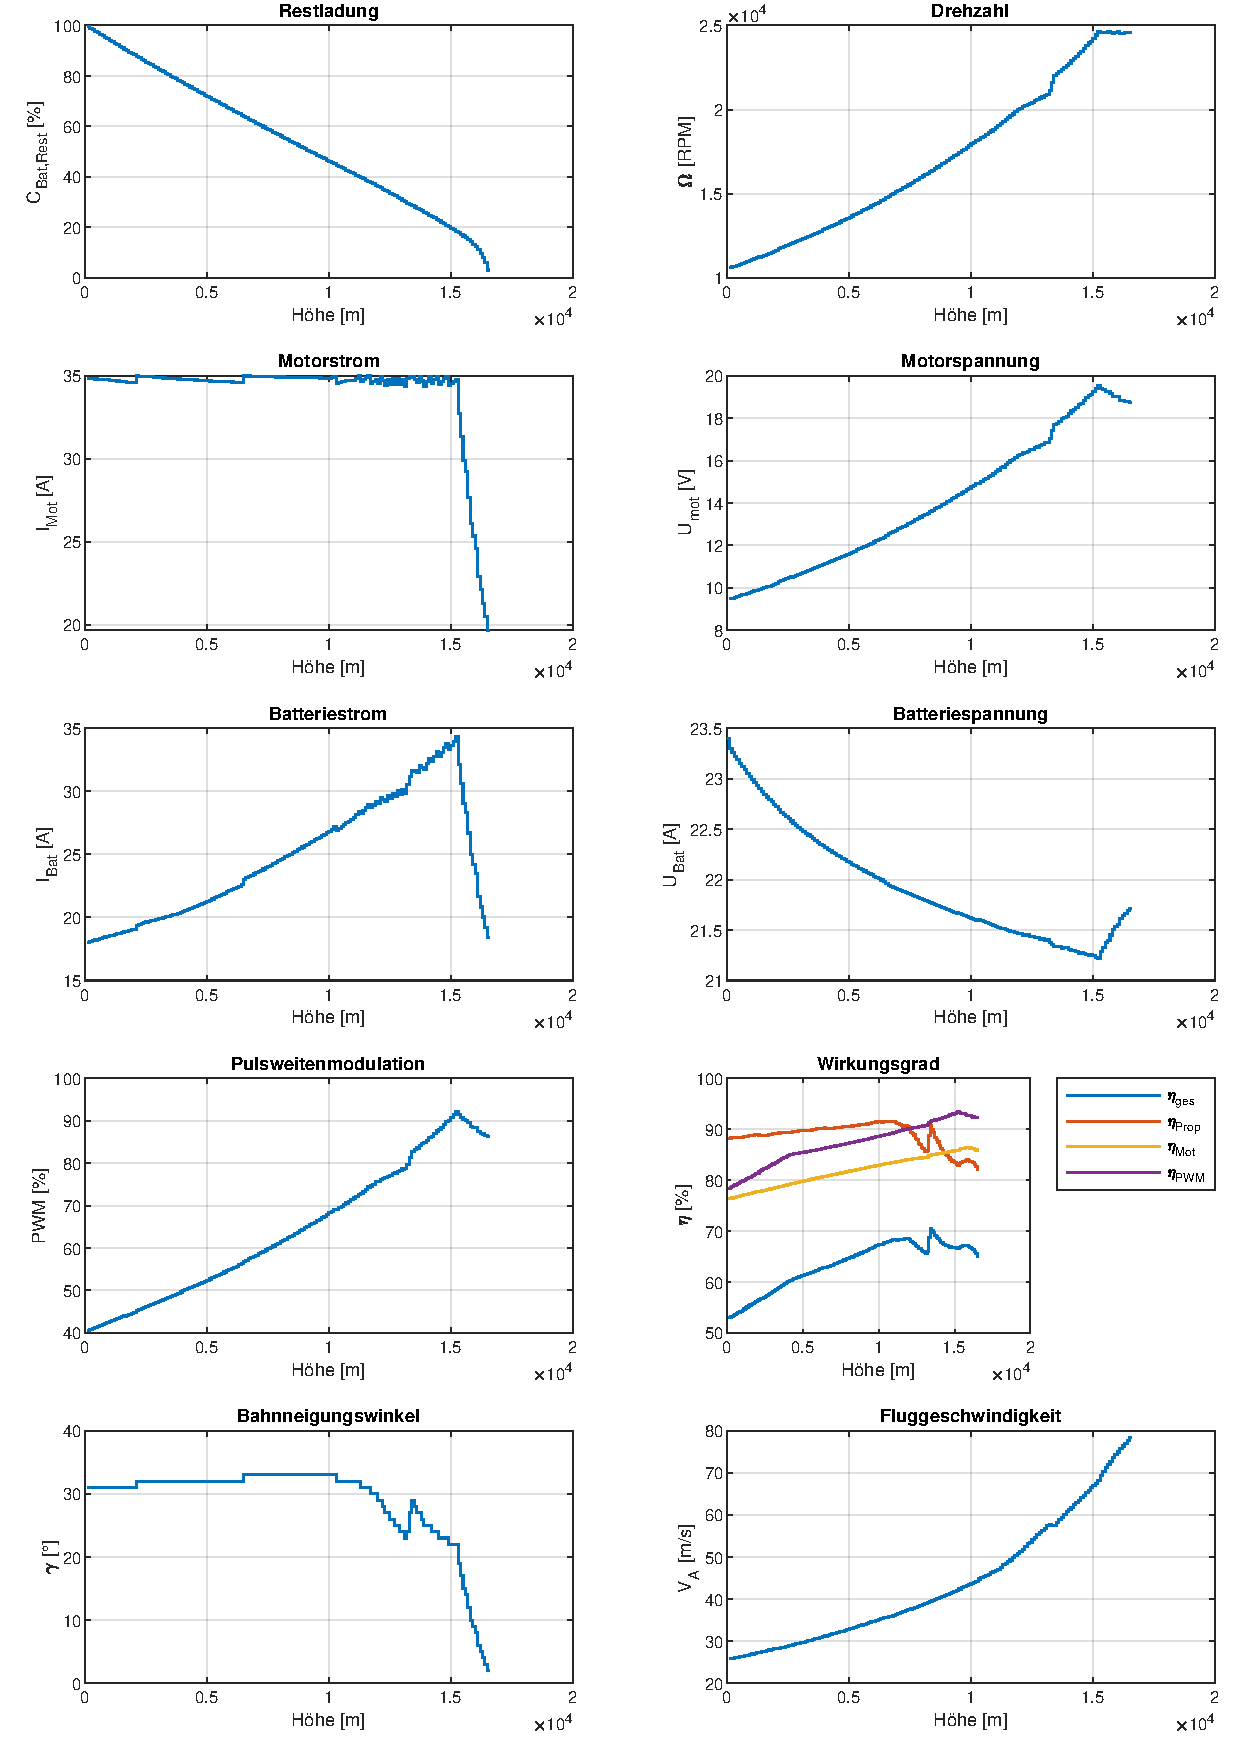
\includegraphics[scale=0.7]{Diagramme/Ausgangskonstellation.pdf}
	\caption{Verlauf der Leistungsparameter über der Höhe für ein Flächenflugzeug mit den in Tabelle \ref{tab:flzg_parameter} definierten Parametern}
	\label{abb:ausgangskonstellation}
\end{figure}

Die gewählte Konstellation erreicht mehr als \SI{13000}{m} Höhe (Vgl. Abb. \ref{abb:ausgangskonstellation}). Der die Höhe begrenzende Faktor ist in diesem Fall die fehlende Leistung zum Aufstieg in noch größere Höhen. Zu Beginn des Steigflugs stellt sich ein optimaler Bahnneigungswinkel von ca. \SI{31}{^\circ} bis \SI{33}{^\star} ein. Dieser Winkel kann bis zu einer Höhe \SI{9800}{m} gehalten werden. Dabei steigt die absolute Fluggeschwindigkeit leicht quadratisch mit dem Produkt aus \ensuremath{\sqrt{\rho^\star/\rho}} an (Vgl. Gleichung \ref{eq:geschw_flaechenflugzeug}). Zu Beginn des Steigfluges wären größere Steigwinkel effizienter, allerdings werden diese durch den maximalen Motorstrom (\ensuremath{I_{max} = \SI{35}{A}}) begrenzt. Ohne diesen würde der Bahnneigungswinkel beinahe linear absinken. Daraus kann geschlossen werden, dass ein Flug mit maximalem Motorstrom im unteren Höhenbereich am effizientesten ist. Der sägezahnartige Verlauf des Motorstroms hängt mit der gewählten Diskretisierung und dadurch rückwirkend mit der Genauigkeit zusammen. Eine genauere Untersuchung dieser Punkte würde zu einem glatten Verlauf des Motorstroms bei \ensuremath{I_{max}} führen. Ebenso würden sich die Verläufe aller anderen Leistungsparameter über der Höhe glätten. Gleichzeitig zum konstanten Motorstrom wächst die Motorspannung linear an, bis diese ab \SI{98000}{m} das Niveau der Batteriespannung erreicht. Damit ist das Verhältnis von \ensuremath{U_{Mot}} und \ensuremath{U_{Bat}} gleich 1 und  die PWM liegt bei \SI{100}{\%}. Ab diesem Zeitpunkt kann die Leistung für die Geschwindigkeit und den Schub bei einem konstanten Steigwinkel nicht mehr aufgebracht werden. Der Zusammenhang ergibt sich daher, dass mit dem Bahnanstellwinkel und der Höhe (indirekt durch die Dichte) der Schub und die Geschwindigkeit steigen (Vgl. Gleichung \ref{eq:schub_flaechenflugzeug} und \ref{eq:schub_flaechenflugzeug}). Außerdem wird der Motor bereits bei Vollast betrieben. Die maximale Motorspannung entspricht hier der maximalen Batteriespannung, die durch die Last von anfänglich \SI{15,5}{V} auf ca. \SI{14.45}{V} einbricht. Der Verlauf des Batteriestroms steht in direktem Zusammenhang mit dem Motorstrom und der Motorspannung. Dies wird aus Gleichung \ref{eq:batteriestrom} ersichtlich. Bei einem konstantem Motorstrom ist  \ensuremath{I_{Bat}} nur von \ensuremath{U_{Mot}} abhängig. Daher der gleiche Verlauf wie bei \ensuremath{U_{Mot}}. Danach ist \ensuremath{U_{Mot}} beinahe konstant und \ensuremath{I_{Bat}} hängt nur noch von \ensuremath{I_{Mot}} ab. Der Verlauf der Drehzahl ist ausschlaggebend für den des Motorspannung. Da die Motorspannung nicht weiter steigen kann und der Motorstrom leicht absinkt, kann die Drehzahl analog zum sinkenden Strom durch die festgelegten Grenzen leicht steigen (Vgl. Gleichung \ref{eq:motorspannung}). Die Maximaldrehzahl kann damit nur noch leicht auf \SI{19000}{RPM} steigen. 
Die Restladung nimmt mit der Höhe linear ab. Erst ab dem Flugzustand mit \SI{100}{\%} PWM nimmt die Restladung der Batterie deutlich schneller ab. Am höchsten Punkt des Aufstiegs können noch min. \SI{20}{\%} Restladung verzeichnet werden.
Der Gesamtwirkungsgrad gliedert sich wie in Kap. \ref{subsec:eta_ges} dargelegt in den Propeller-, den Motor- und den Motorreglerwirkungsgrad. Daher folgt er zeitgleich den anderen Wirkungsgraden. Der Propellerwirkungsgrad steigt mit der Höhe an. Ausschlaggebend hierfür ist die steigende Geschwindigkeit und die Drehzahl (Vgl. Gleichung \ref{eq:eta_prop}). Während der noch flugleistungstechnisch erreichbare Bahnneigungswinkel abfällt, steigt die Bahngeschwindigkeit und der Propellerwirkungsgrad. Über Gleichung \ref{eq:geschw_flaechenflugzeug} nimmt mit steigendem Bahnneigungswinkel die Fluggeschwindigkeit ab. Da dieser jedoch nun absinkt, nimmt damit auch die Fluggeschwindigkeit zu. Da die Motorspannung bereits ihr Maximum erreicht hat, kann die Propellerdrehzahl nur noch leicht mit der abnehmenden Dichte und somit geringer werdenden Widerstandskräften ansteigen (Vgl. Gleichung \ref{eq:motorspannung}. Dabei nimmt auch das Propellerdrehmoment ab (Ergebnis aus Gleichung \ref{eq:motorstrom}). Bei einer gleichermaßen steigenden absoluten Fluggeschwindigkeit, steigt die Strahlleistung des Propellers (Vgl. Gleichung \ref{eq:strahlleistung}). Als Konsequenz steigt der Propellerwirkungsgrad.
Dies gilt auch für den Motorwirkungsgrad. Dieser steigt mit einer anwachsenden Propellerdrehzahl und -drehmoment (Vgl. Gleichung \ref{eq:eta_mot}). Außerdem nehmen die durch den Innenwiderstand und den Leerlaufstrom verursachten Verluste anteilig am Motorstrom und der -spannung ab (Vgl. Gleichung \ref{eq:motorstrom} und \ref{motorspannung}), die mit zunehmender Höhe auch zunehmen. Der Grund hierfür liegt in der Annahme, dass diese beiden Motorkenngrößen für jeden Motorzustand als konstant angesehen werden. Der Wirkungsgrad des ESC steigt simultan mit der Höhe und der PWM. Mit steigender PWM nehmen auch die Verluste innerhalb des Motorreglers ab (Vgl. Gleichung \ref{eq:eta_pwm}). Deutlich zu erkennen ist eine Abnahme aller Wirkungsgrade, wenn die PWM \SI{100}{\%} erreicht und damit der Motorstrom sowie der Bahnneigungswinkel absinken. Dies ist ein Indiz für den Beginn eines ineffizienteren Flugzustandes.



% Die maximale Motorspannung entspricht ab \SI{11400}{m} Flughöhe der maximalen Batteriespannung, die durch die Last von anfänglich \SI{15,6}{V} auf ca. \SI{14.7}{V} einbricht. Der Verlauf des Batteriestroms steht in direktem Zusammenhang mit dem Motorstrom und der Motorspannung. Dies wird aus Gleichung \ref{eq:batteriestrom} ersichtlich. Bei einem beinahe konstantem Motorstrom ist \ensuremath{I_{Bat}} fast ausschließlich von \ensuremath{U_{Mot}} abhängig. Daher der gleiche Verlauf wie bei \ensuremath{U_{Mot}}. Danach ist \ensuremath{U_{Mot}} konstant und \ensuremath{I_{Bat}} hängt nur noch von \ensuremath{I_{Mot}} ab. 
%Der Verlauf der Drehzahl ist ausschlaggebend für den des Motorspannung. Da die Motorspannung nicht weiter steigen kann und der Motorstrom leicht absinkt, kann die Drehzahl analog zum sinkenden Strom durch die festgelegten Grenzen leicht steigen (Vgl. Gleichung \ref{eq:motorspannung}). Die Maximaldrehzahl ist damit auf \SI{12000}{RPM} begrenzt. 

%Zu Beginn des Steigfluges wären größere Steigwinkel effizienter, allerdings werden diese durch den maximalen Motorstrom begrenzt. Ohne diese würde der Bahnneigungswinkel beinahe linear absinken. Daraus kann geschlossen werden, dass ein Flug mit maximalem Motorstrom im unteren Höhenbereich am effizientesten ist. Der sägezahnartige Verlauf der Motorspannung hängt mit der gewählten Diskretisierung / Genauigkeit zusammen. Eine genauere Untersuchung dieser Punkte würde zu einem glatten Verlauf des Motorstroms bei \ensuremath{I_{max}} führen. Ebenso würde sich der Verlauf aller anderen Kurven glätten. Gleichzeitig zum konstanten Motorstrom wächst die Motorspannung linear an, bis sie ab \SI{11400}{m} das Niveau der Batteriespannung erreicht. Damit ist die PWM bei \SI{100}{\%}. Ab diesem Zeitpunkt kann nicht mehr mit maximalem Motorstrom geflogen werden, \textcolor{red}{wodurch folglich der Motorspannung und der Bahnneigungswinkel simultan abfallen}. 
%Der Zusammenhang ergibt sich daher, dass mit dem Bahnanstellwinkel der Schub und die Geschwindigkeit steigen (Vgl. Gleichung \ref{eq:schub_flaechenflugzeug} und \ref{eq:schub_flaechenflugzeug}). Die im Anschluss aus dem Kennfeld interpolierte Drehzahl fließt direkt in den Motorstrom ein (Vgl. Gleichung \ref{eq:motorstrom}). Bedingt durch die mit dem Winkel und der Höhe (indirekt durch die Dichte) steigende Geschwindigkeit, können die Steigwinkel leistungsbedingt nicht mehr aufgebracht werden. Die maximale Motorspannung entspricht hier der maximalen Batteriespannung, die durch die Last von anfänglich \SI{15,6}{V} auf ca. \SI{14.7}{V} einbricht. Der Verlauf des Batteriestroms steht in direktem Zusammenhang mit dem Motorstrom und der Motorspannung. Dies wird aus Gleichung \ref{eq:batteriestrom} ersichtlich. Bei konstanten Motorstrom ist die \ensuremath{I_{Bat}} nur von \ensuremath{U_{Mot}} abhängig. Daher der gleiche Verlauf wie bei \ensuremath{U_{Mot}}. Danach ist \ensuremath{U_{Mot}} konstant und \ensuremath{I_{Bat}} hängt nur noch von \ensuremath{I_{Mot}} ab.

%Gleichzeitig steigt der Motorstrom leicht, da für einen konstanten Bahnneigungswinkel der benötigte Schub konstant bleibt (Vgl. Gleichung \ref{eq:schub_flaechenflugzeug}), aber mit abnehmenden Dichte das Drehmoment zunimmt. Noch stärker als der Motorstrom steigt die Motorspannung linear an, bis sie das Niveau des Batteriestroms erreicht. Damit ist das Verhältnis von \ensuremath{U_{Mot}} und \ensuremath{U_{Bat}} gleich 1 und  die PWM liegt bei \SI{100}{\%}. Ab diesem Zeitpunkt kann \textcolor{red}{leistungsbedingt} die Geschwindigkeit und Schub für einen konstanten Steigwinkel nicht mehr gehalten werden. Folglich sinkt der Bahnneigungswinkel, da für ein Höhenintervall die absolute Fluggeschwindigkeit und analog die Steiggeschwindigkeit \ensuremath{V_H} mit einem mit einem  größeren Bahnneigungswinkel sinkt (Vgl. Gleichung \ref{eq:geschw_flaechenflugzeug}).


\subsection{Einflussfaktoren auf das Flächenflugzeug}
Die zu variierenden Parameter des Flächenflugzeugs sind diejenigen Leistungsparameter, die das Fluggerät qualifizieren. Das sind die Motor-Propeller-Kombination, die Propelleranzahl, die Gleitzahl, die Auslegungsgeschwindigkeit und der Penalty-Faktor.

\subsubsection{Motor-Propeller Kombination}
\label{subsubsec:mot_prop_kombi}
Die Motor-Propeller-Kombination beeinflusst entscheidend das Leistungsverhalten von elektrisch, propellergetriebenen Fluggeräten. Mit dem in Tab. \ref{tab:flzg_parameter} aufgeführten Motor mit einem Gewicht von \SI{106}{g} und einem \ensuremath{K_V}-Wert von \SI{1390}{RPM/V} sind bereits sehr hohe Flughöhen erreichbar. Bei Verwendung des gleichen Propellers, einem 9x7 Propeller, und der Variation des \ensuremath{K_V}-Wertes, zeigen die Motoren mit einem größeren \ensuremath{K_V}-Wert ein besseres Flugverhalten (Vgl. Abb. \ref{abb:flaechenflzg_mot_prop}).\\
Die optimale Flugweise des Flächenflugzeuges ist für jede Art des Motors mit gleichem Gewicht identisch. Zuerst wird solange mit maximalem Motorstrom geflogen, bis die Schubhebelstellung \SI{100}{\%} erreicht. Danach sinkt der Bahnneigungswinkel während die Steiggeschwindigkeit steigt. Die maximale Höhe ist erreicht, wenn der noch fliegbare Steigwinkel Null erreicht und kein Steigflug mehr möglich ist. Der Steigwinkel legt dabei in einem Bereich von \SI{15}{^\circ} und \SI{20}{^\circ}. \\
Mit dem \ensuremath{K_V}-Wert steigt ebenso die maximale Höhe (Vgl. Abb. \ref{abb:flaechenflzg_mot_prop}). Den größten Einfluss auf die Flugleistung hat der \ensuremath{K_V}-Wert auf die Motorspannung. Hier gilt, dass bei einer annähernd gleichen Drehzahl die Motorspannung mit dem \ensuremath{K_V}-Wert sinkt. Der Grund dafür liegt in der Definition dieses Motorkennwertes.\\

\begin{figure}[H]
\centering
	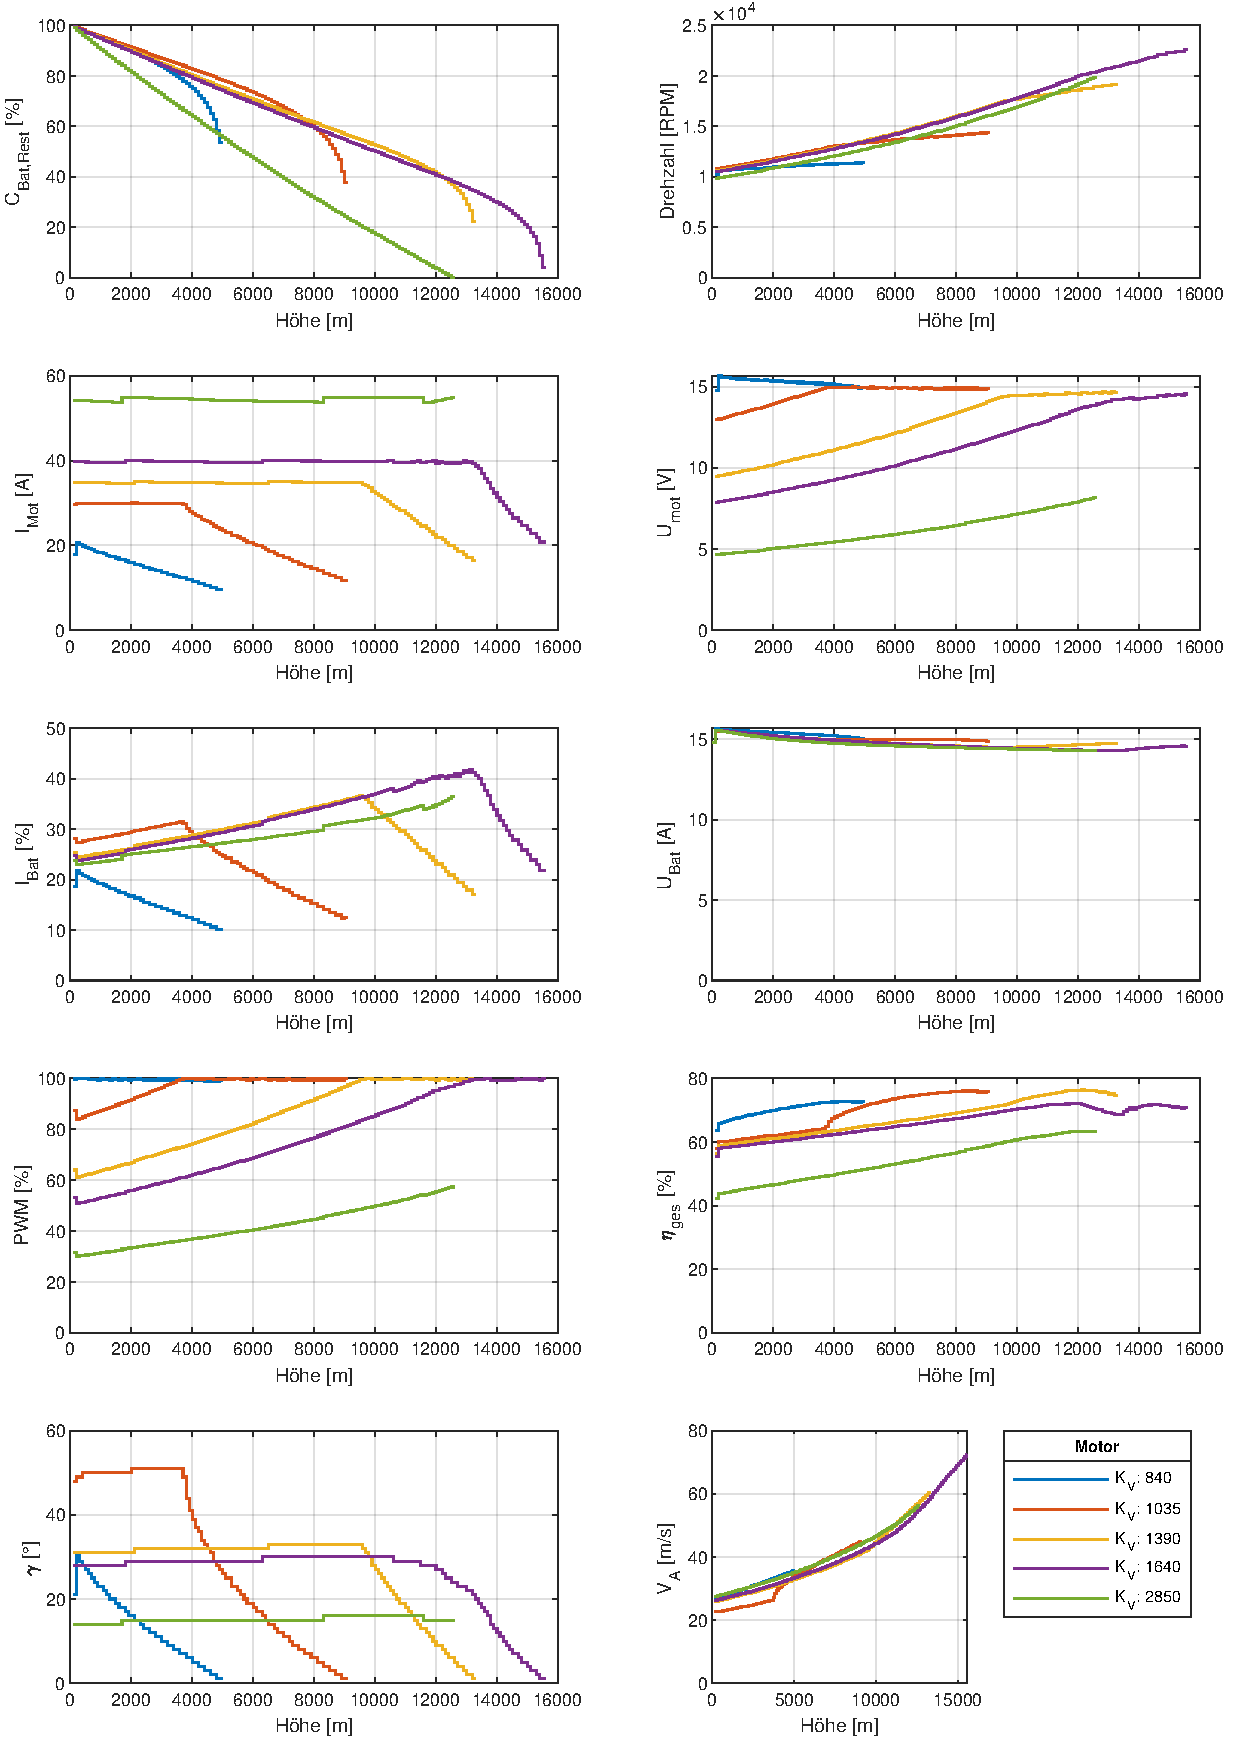
\includegraphics[scale=0.7]{Diagramme/Flaechenflzg_Mot_Prop.pdf}
	\caption{Einfluss der Motor-Propeller-Kombination auf die Flugleistungen eines Flächenflugzeugs (\ensuremath{m_{Mot}} = \SI{106}{g}, Propeller = 9x7)}
	\label{abb:flaechenflzg_mot_prop}
\end{figure}

Der \ensuremath{K_V}-Wert ist ein Kennwert für die Anzahl der Umdrehungen pro Minute pro Volt im Leerlauf. Ein hoher \ensuremath{K_V}-Wert bedeutet nun im Umkehrschluss, dass bei einer hohen Drehzahl die Spannung geringer ist als für einen Motor mit einem vergleichsweise niedrigem \ensuremath{K_V}-Wert. Gleichzeitig sinkt allerdings das Verhältnis von Drehmoment pro Ampere, das der \ensuremath{K_M}-ausdrückt  \cite[S.35 und S.42-43]{Buchi.2013}. Es gilt die Beziehung
\begin{equation}
	K_M = 1/K_V\cdot 30/\pi.
\end{equation}
Ein Motor mit hohem \ensuremath{K_V}-Wert muss daher einen hohen Dauermotorstrom besitzen, um gute Flugleistungen zu erzielen (Vgl. Abb. \ref{abb:flaechenflzg_mot_prop}). Dies ergeben auch die Ergebnisse in Abb. \ref{abb:flaechenflzg_mot_prop}. Durch diese Abhängigkeit wird auch die PWM beeinflusst. Der Motor mit einem \ensuremath{K_V} von \SI{840}{RPM/V} erreicht durch seine hohe Motorspannung deutlich schneller das Niveau der Batteriespannung. Somit wird auch frühzeitiger das Absinken des Bahnneigungswinkels eingeleitet, weil die maximale Motorleistung erreicht ist. Für Motoren mit einem niedrigeren \ensuremath{K_V}-Wert bedeutet dies auch gleichzeitig das Ende des Steigfluges. Wieder anders ist dieser Zusammenhang für Motoren mit einem hohen \ensuremath{K_V}-Wert. Hier wird \SI{100}{\%} PWM erst bei deutlich größeren Höhen erreicht, weshalb folglich der optimale Bahnneigungswinkel erst später nicht mehr gehalten werden kann und danach abflacht. Den Steigflug begrenzt in diesem Fall die Restladung. Dabei nimmt die Restladung für kleinere \ensuremath{K_V}-Werte nicht so schnell ab wie dies für große der Fall ist. Die kann auf den höheren Gesamtwirkungsgrad und im Detail auf den höheren \textcolor{red}{Motorreglerwirkungsgrad zurückgeführt werden auch ein höherer Motorwirkungsgrad bei höherer Spannung}. Durch die deutlich höhere Pulsweitenmodulation ist der Wirkungsgrad des Motorreglers entsprechend höher (Vgl. Gleichung \ref{eq:eta_pwm}. Außerdem sind die Verluste durch Temperatur  sowie Innenwiderstand oder Leerlaufstrom für einen Motoren mit niedrigem \ensuremath{K_V}-Wert geringer.\\
An dieser Stelle ist auch die Motor-Propeller Kombination zu beachten. Der Motor mit einem \ensuremath{K_V}-Wert von 2850 erzielt mit dem 9x7 Propeller zwar etwas schlechtere Flugleistungen, erreicht mit einem 6x4 Propeller jedoch noch größere Höhen (siehe Anhang). Zusammengenommen zeigt sich, dass mit geringer werdenden \ensuremath{K_V}-Wert, also einem langsamer, aber mit höherem Drehmoment drehender Motor, der optimale Durchmesser des Propellers in reziproker Weise steigt bei einem gleichen Verhältnis zwischen Durchmesser und Steigung. Dies kann relativ einfach mit den Angaben der Hersteller zu der besten Motor-Propeller-Kombination verglichen werden. Nach \cite{Wall.2015} erhöht sich der Wirkungsgrad eines Rotors mit größer werdenden Durchmesser. 
Mit den oben gemachten Aussagen zu einer Motor-Propeller-Kombination wird im Folgenden der Propeller an die Wahl der Motoren angepasst.
\textcolor{red}{hier anbringen, dass Effizienz von einem Motor mit geringem kV höher ist, weniger Verluste und weniger Erhitzung, 
http://rcboats.kiwi/index.php/ct-menu-item-15/ct-menu-item-31/ct-menu-item-43}


\subsubsection{Anzahl der Motoren und Propeller}
Während die Leistung der Motoren mit gleichem Gewicht wenig Einfluss auf den optimalen Steigwinkel hat, ändert sich dies bedeutend mit der Anzahl der Motoren. Schon mit einer Steigerung der Motorenanzahl auf 2 verändert sich der optimale Steigwinkel zu \SI{90}{^\circ}. Die dazu zugehörige Steiggeschwindigkeit liegt hierbei beim Maximum der Steiggeschwindigkeitsiterationsweite. Dies ist solange der optimale Betriebspunkt bis der Steigwinkel von \SI{55}{^\circ} optimaler ist.
Ebenfalls wie oben beschrieben ist dieser Zustand so lange fliegbar bis der Motorstrom auf dem Niveau des Batteriestroms und damit \SI{100}{\%} der PWM erreicht ist. Ab diesem Punkt steigt der Bahnneigungswinkel wieder an, da für einen Höhenschritt die Fluggeschwindigkeit mit Winkel sinkt. Alle anderen Größen verhalten sich analog zum oben beschriebenen Zustand (Vgl. Kap. \ref{subsec:erste_untersuchung}). Ein vergleichbares Flugverhalten ist bei einer Erhöhung der Anzahl auf 4 zu beobachten.
Mit der Propelleranzahl verringert sich der Schub, der pro Propeller aufgebracht werden muss und damit auch die vom Motor benötigte Leistung. Folglich erhöht sich auch der Leistungsüberschuss. Dies resultiert auf der anderen Seite in einer höheren Belastung der Batterie. Beachtlich ist auch, dass die Batterie am TOC noch beinahe \SI{50}{\%} Restladung besitzt. Dies ist signifikant mehr als beim Quadrocopter. Bei diesem ist der Steigflug beendet, wenn die Batterie leer ist. Beim Flächenflugzeug ist die Motorleistung der limitierende Parameter.

\begin{figure}[H]
\centering
	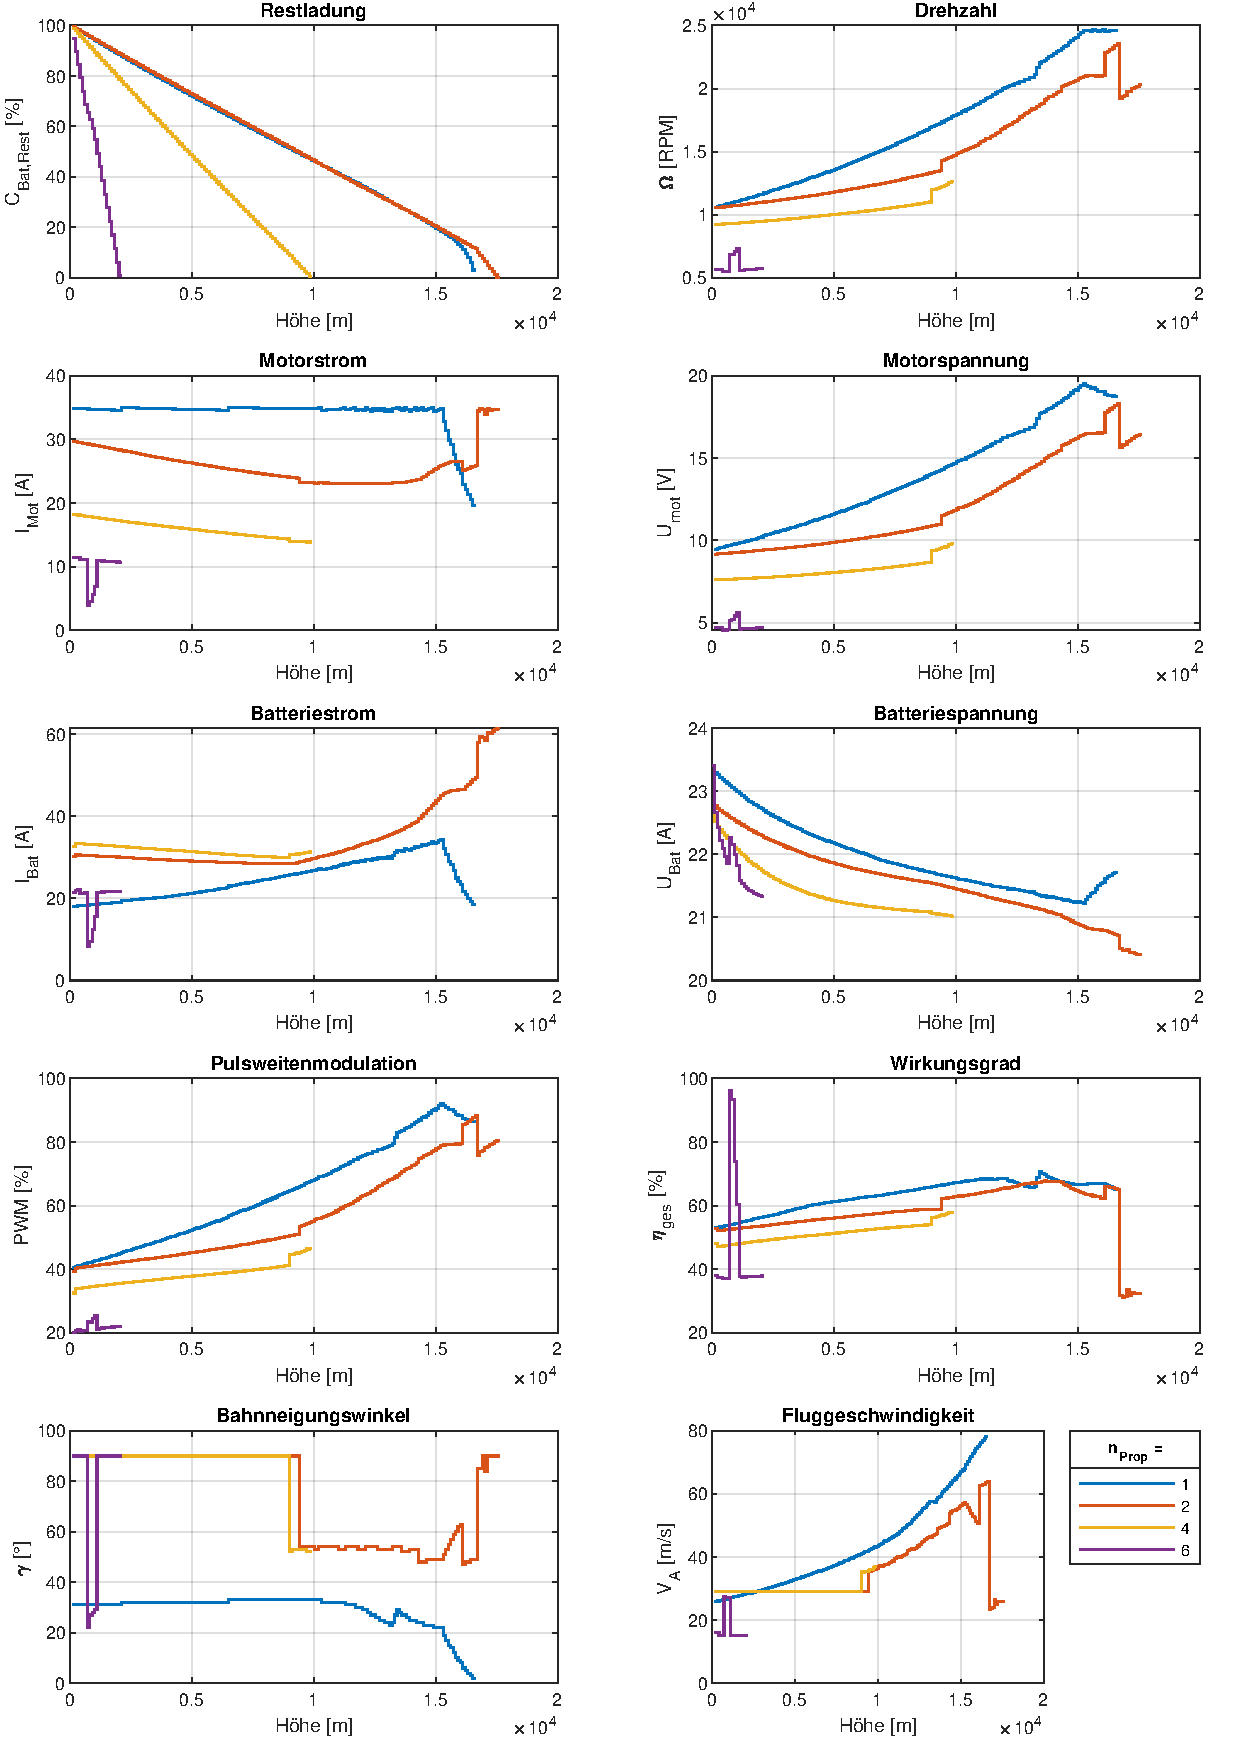
\includegraphics[scale=0.7]{Diagramme/Flaechenflzg_n_prop.pdf}
	\caption{Einfluss der Propelleranzahl auf die Flugleistungen eines Flächenflugzeugs (\ensuremath{m_{Mot}} = \SI{106}{g}, Propeller = 9x7)}
	\label{abb:flaechenflzg_mot_prop}
\end{figure}


\subsubsection{Gleitzahl}
Mit einer Verringerung der Gleitzahl geht auch eine Verringerung der maximalen Höhe mit einher und vice versa. Eine entsprechend hohe Gleitzahl beudeuted gleichzeitig auch eine entsprechend hohe aerodynamische Güte (Vgl. \cite[S.34]{Scheiderer.2008}). Dazu sinkt der Widerstand im Vergleich zum Auftrieb, sodass für ein Flächenflugzeug mit einer höheren Gleitzahl für den gleichen Auftrieb weniger Leistung zur Kompensation des Widerstandes aufgebracht werden muss. Als Konsequenz dessen steht mehr Leistung für das Steigen zur Verfügung. Mit der Gleitzahl steigt ebenso der optimale Steigwinkel. Als Grund dafür kann wieder die verringerte Widerstandsleistung angeführt werden. Zusätzlich sinkt die Zeit zum Überwinden einer Höhendifferenz mit steilerem Winkel. Einen Änderung der Gleitzahl hat nur einen Einfluss der auf die Restladung, die Batteriespannung und den Bahnneigungswinkel. Eine geringe Gleitzahl bedeutet einen stärkeren Einbruch der Batteriespannung, da wiederum im für den gleichen Auftrieb mehr Widerstand kompensiert werden muss. Auffällig ist noch Verbesserungszunahme der Flugleistungen mit der Gleitzahl. Diese Änderung ist im Bereich von 4 auf 10 deutich ausgeprägter als von 20 auf 50, obwohl dies mindestens einer Verdoppelung der Gleitleistung gleichkommt.
\begin{figure}[H]
\centering
	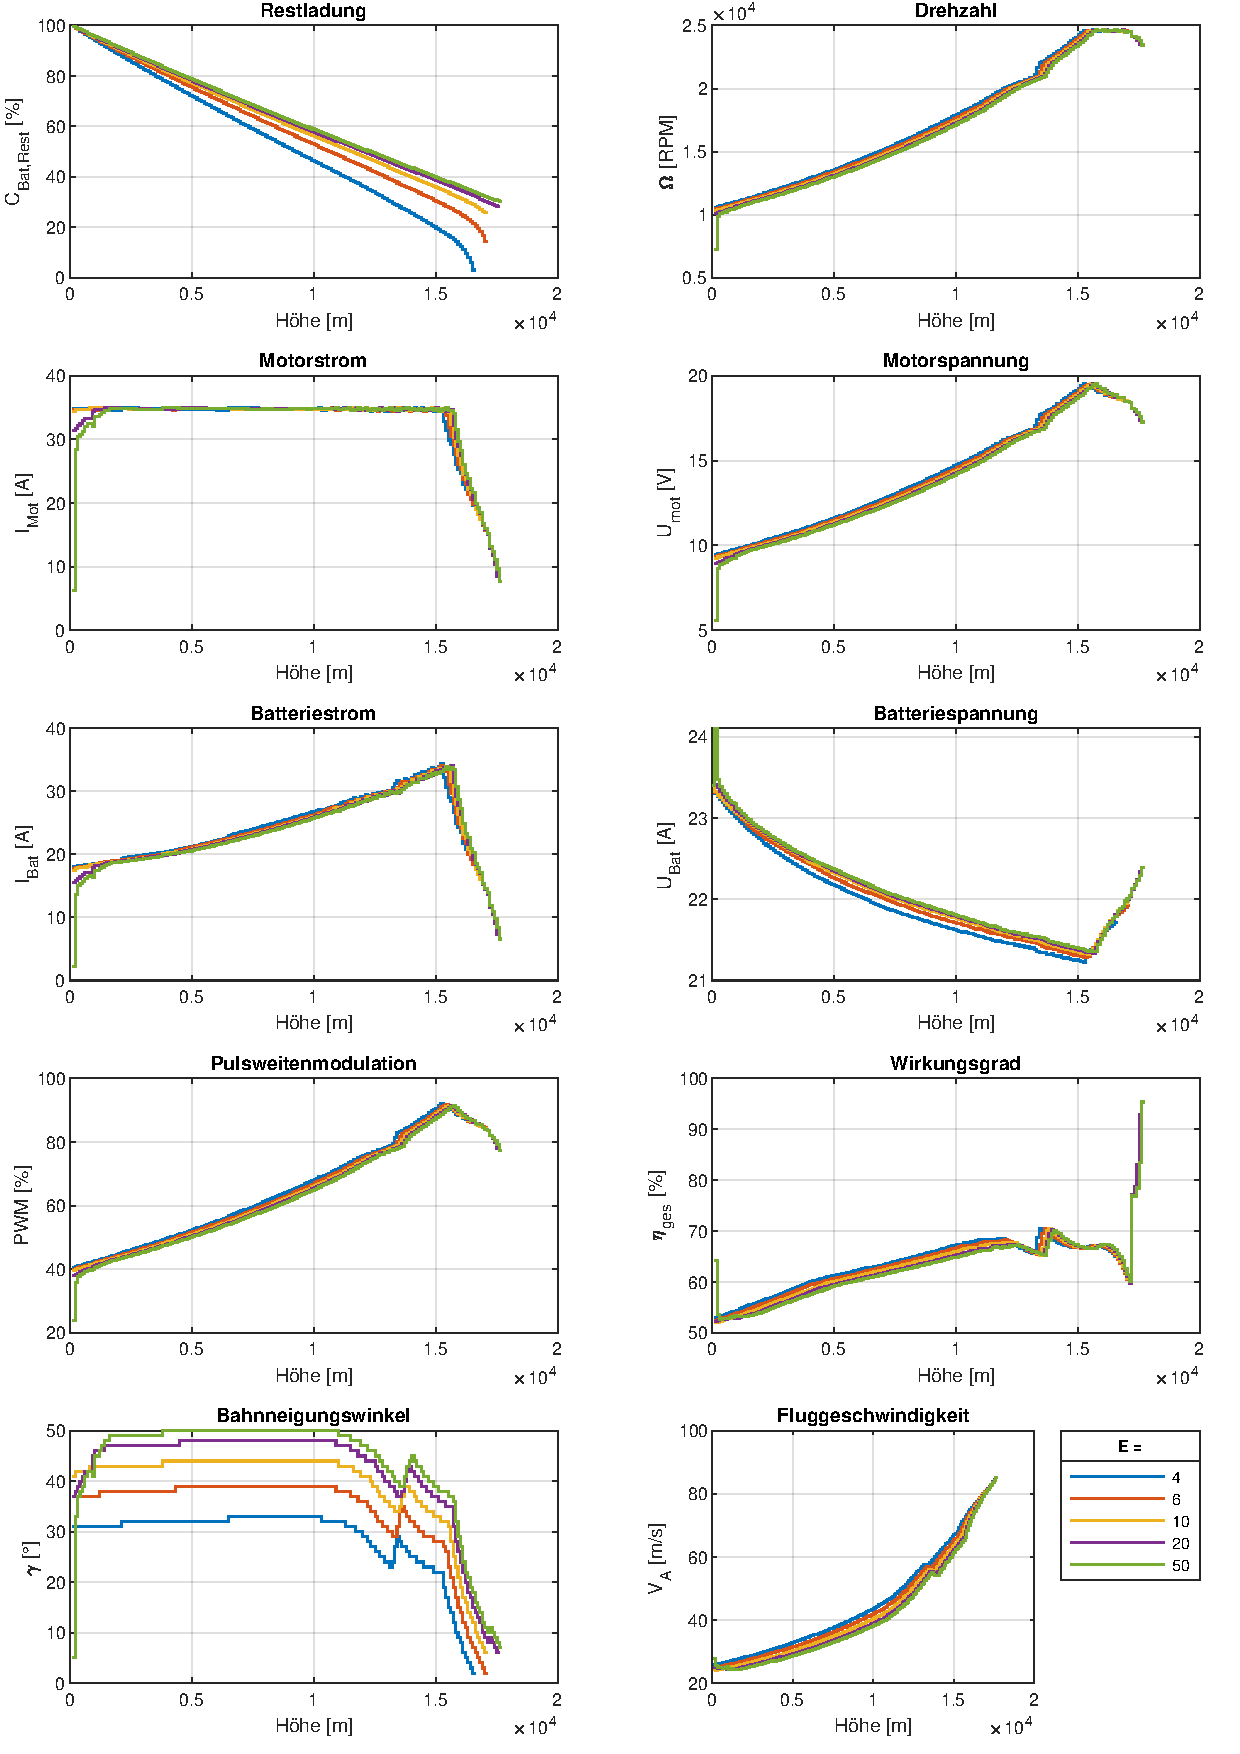
\includegraphics[scale=0.7]{Diagramme/Flaechenflzg_E.pdf}
	\caption{Einfluss der Gleitzahl auf die Flugleistungen eines Flächenflugzeugs}
	\label{abb:gleitzahl}
\end{figure}


\subsubsection{Auslegungsgeschwindigkeit}
Die Auslegungsgeschwindigkeit hat einen bedeutenden Einfluss auf die erreichbare Höhe. Da für den Steigflug ein Flug mit konstanten Auftriebsbeiwert vorausgesetzt wird, erhöht sich aufgrund dessen die absolute Fluggeschwindigkeit mit der Höhe und größerem Bahnneigungswinkel (Vgl. Gleichung \ref{eq:geschw_flaechenflugzeug}).
Ist die Auslegungsgeschwindigkeit gering, so wächst sie absolut gesehen mit der Höhe nicht so stark wie hohe Geschwindigkeiten. Eine geringer gewählte Auslegungsgeschwindigkeit im Horizontalflug bedeutet daher auch, dass länger mit maximalen Motorstrom geflogen werden kann, bevor die Motorspannung die Batteriespannung erreicht und somit das Absinken des Steigwinkels einleitet.
Da mit der Auslegungsgeschwindigkeit auch die Geschwindigkeit mit der Höhe steigt, sind für hohe Geschwindigkeiten Propeller mit hohem Pitch vom Vorteil.
Ein Optimum zeichnet sich bei \SI{75}{km/h} aus. Es kann festgehalten werden, dass mit der Auslegungsgeschwindigkeit der Bahnneigungswinkel abnimmt, da die Steigzeit bei einer höheren Geschwindigkeit und geringerem Bahnneigungswinkel sich kaum ändert. Außerdem wird schneller \SI{100}{\%} PWM erreicht und damit gleichzeitig die Motorspannung begrenzt und der Flug mit maximalen Motorstrom beendet. Außerdem nimmt mit der Motorspannung der Zuwachs der Propellerdrehzahl ab. Weiterhin ist ein Zuwachs des Gesamtwirkungsgrades sowie der Bahngeschwindigkeit zu verzeichnen. Bei hohen Geschwindigkeiten begrenzt der mögliche Steigwinkel \ensuremath{\gamma} den Steigflug im Gegensatz zu der Begrenzung durch die Restladung bei niedrigen Auslegungsgeshwindigkeiten. Das schnelle Absinken von \ensuremath{\gamma} am Ende des  bedeutet für alle Auslegungen ein ineffizientes Manöver, da damit die Flugzeit für eine Höhenschritt ansteigt und auch einer deutlich höhere Energieentnahme der Batterie mit sich zieht.

\begin{figure}[H]
\centering
	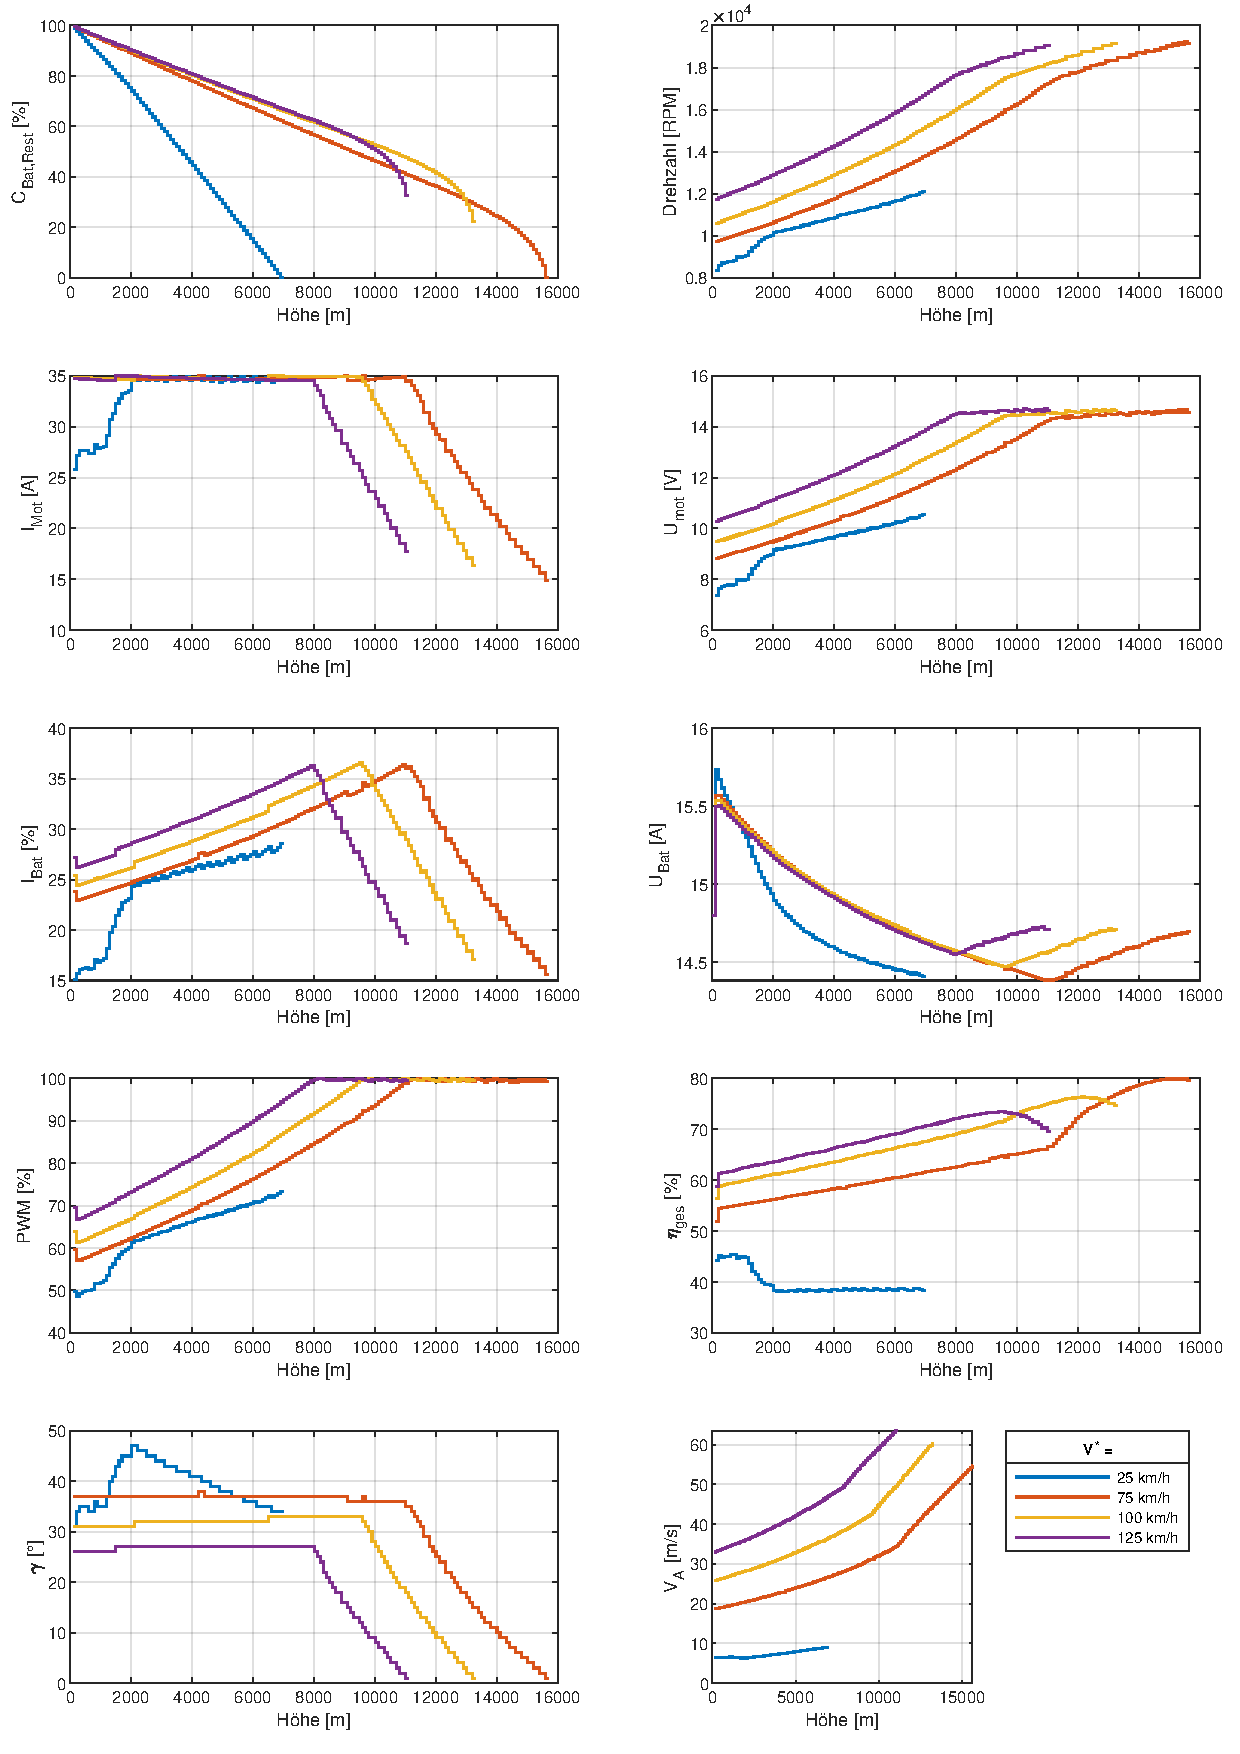
\includegraphics[scale=0.8]{Diagramme/Flaechenflzg_Vstern.pdf}
	\caption{Einfluss der Auslegungsgeschwindigkeit auf die Flugleistungen eines Flächenflugzeugs}
	\label{abb:vstern}
\end{figure}



\subsubsection{Penaltyfaktor}
Im Vergleich von einem Flächenflugzeug mit einem Multicopter muss bei gleichem Gesamtgewicht die unterschiedliche Verteilung der Gewichtskomponenten berücksichtigt werden. Für ein Flugzeug ist das Strukturgewicht von Flügeln und Rumpf sowie den Steuerungselementen bedeutend größer als das von einem Multicopter. Ein Penaltyfaktor von 1 entspricht daher wie oben beschrieben einer sehr optimistischen Einschätzung, wenn beide Strukturgewichte bei einem gleichen Gesamtgewicht äquivalent sind. Um realistischere Ergebnisse für ein Flächenflugzeug zu erreichen, wird der Penaltyfaktor schrittweise erhöht. Dabei verringert sich auch die maximal erreichbare Höhe. Dies hängt damit zusammen, dass ein Penaltyfaktor größer als 1 die zur Verfügung stehende Batteriemasse und folglich die Batteriekapazität reduziert.

\begin{figure}[H]
\centering
	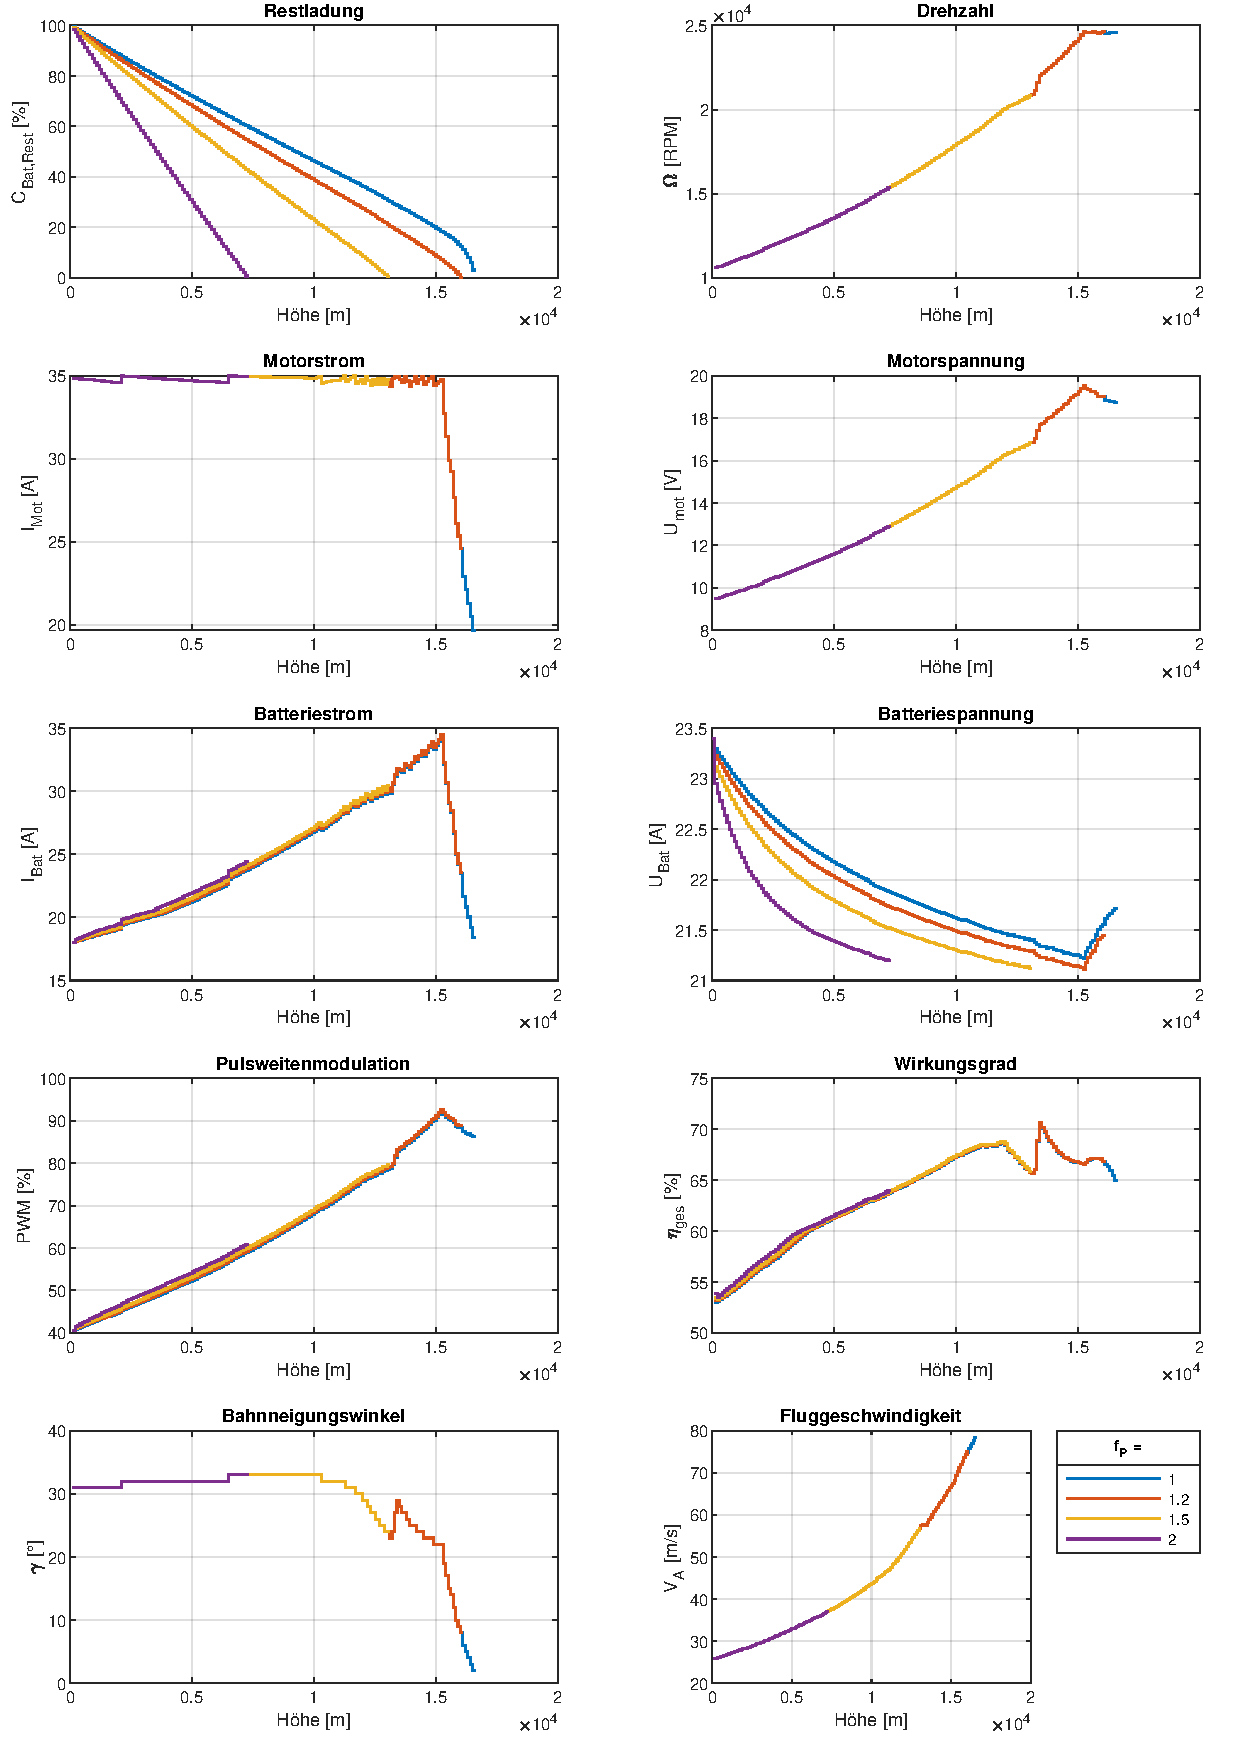
\includegraphics[scale=0.7]{Diagramme/Flaechenflzg_fp.pdf}
	\caption{Einfluss des Penalty-Faktors auf die Flugleistungen eines Flächenflugzeugs}
	\label{abb:fp}
\end{figure}


%\subsubsection{Motor-Propeller-Kombination}
%Die Motor-Propeller-Kombination beeinflusst entscheidend das Leistungsverhalten von elektrisch, propellergetriebenen Fluggeräten. Für jeden Motor werden vom Hersteller Propeller für einen bestimmten Anwendungsfall vorgegeben, mit dem optimale Leistungen erbracht werden können. Die Propellergröße hängt von der Leistung des Motors ab und von dem Auslegungsfall. Es zeigt sich, dass je stärker der Motor ist, desto größer ist der optimale Radius. Prinzipiell können auch kleinere Propeller verwendet werden. Aufgrund der Motorleistung ist der Pitch deshalb groß zu wählen, um den erforderlichen Schub zu liefern. Wird der Radius weiter vergrößert, so verringert sich der optimale Pitch. Außerdem sind Motoren mit niedrigen \ensuremath{K_V}-Werten bei gleichem Motorgewicht zu bevorzugen. Dies liegt in der Tatsache begründet, dass der \ensuremath{K_V}-Wert direkt den Motorstrom beeinflusst und ein hoher Wert diesen entsprechend zu Beginn des Fluges bereits stark erhöht. Zudem steht ein hoher \ensuremath{K_V} für eine hohe Maximaldrehzahl des Motors, aber für entsprechend weniger Drehmoment. Das gleiche gilt umgekehrt. 



%\subsubsection{Anzahl der Motoren}
%Noch bessere Ergebnisse können mit 2 Motoren erreicht werden, die  einen niedrigen \ensuremath{K_V}-Wert besitzen, aber ein hohes Leistungsgewicht. Mit dieser Konstellation sind Flughöhen bis zu \SI{15000}{m} möglich. In diesem Fall ist nicht der Flug mit maximalen Motorstrom am effizientesten sonder ein Flug mit konstantem Steigwinkel von ca. \SI{60}{^\circ}. Dabei sinkt der Motorstrom in diesem Zustand leicht, da das Drehmoment mit der Höhe abnimmt. Ebenfalls wie oben ist beschrieben ist dieser Zustand so lange fliegbar bis der Motorstrom auf dem Niveau des Batteriestroms und damit \SI{100}{\%} der PWM erreicht ist. Ab diesem Punkt steigt der Bahnneigungswinkel wieder an, da für einen Höhenschritt die Fluggeschwindigkeit mit Winkel sinkt. Alle anderen Größen verhalten sich analog zum oben beschriebenen Zustand. 
%Mit der Propelleranzahl verringert sich der Schub, der pro Propeller aufgebracht werden muss und damit auch die vom Motor benötigte Leistung. Folglich erhöht sich auch der Leistungsüberschuss. Dies resultiert auf der anderen Seite in einer höheren Belastung der Batterie.


\subsection{Ergebnisse des Vergleichs} 
Im direkten Vergleich weist das Flächenflugzeug eine größere maximale Flughöhe auf. Besonders mit hohen Gleitzahlen, mehreren Motoren und einer guten Kombination aus Motor und Propeller wird dieser Vorteil ersichtlich. Unter Berücksichtigung von zusätzlichen Widerständen und des einfachen Modells ist dieser Vorteil gerade wieder hinfällig sprich der zusätzliche Höhengewinn schwindet zu Null, wenn man die Widerstände berücksichtigt. Weiterhin erweist sich das Flächenflugzeug als bereits in den möglichen Maßen im Rahmen dieses Modells als optimiert. Die Steiggeschwindigkeit ist in Bezug auf den Auslegungszustand und einem Flug bei Auslegungsgleitzahl optimal. Außerdem wird der Steigwinkel für jeden Höhenabschnitt optimiert und eine gute Kombination von Motor und Propeller ist bereits gegeben. Schlussendlich ist damit der Spielraum für weitere Verbesserungen eingeschränkt. Hingegen zeigt der Quadrocopter in dieser Hinsicht noch Potenzial. Ein zu untersuchender Punkt ist noch die Abkehr von einer konstanten Steiggeschwindigkeit hin zu einer kontinuierlichen Optimierung dieser mit der Höhe. \\
Wird für das Flugzeug außerdem eine Konstellation von mehr als einem Motor gewählt, neigt das Flugzeug dazu in einem \SI{90}{^\circ} Winkel zu steigen. Damit zeigt sich die optimale Flugweise in einem vertikalen Steigflug. Hierbei werden nichtsdestotrotz wieder viel Vereinfachungen getroffen und Verluste nicht berücksichtigt. Die Vorteile eines Flächenflugzeuges zeigen sich auch nur stark bei einem Penalty-Faktor nahe bei 1. Dies muss als unrealistisch angesehen werden. Besonders im Bezug auf eine hohe Gleitzahl geht diese Anforderung mit einer hohen Flügelstreckung und damit mit einem hohen Strukturgewicht einher. Somit ist es zwingend notwendig den Penalty-Faktor zu erhöhen. Letztendlich verschwindet damit der Vorteil gegenüber einem Multicopter. 
In der Berechnung der Flächenflugzeugaerodynamik bleibt der Einfluss von Seitenwinden unberücksichtigt, da Seitenwinde nur die Strecke über Grund beeinflussen nicht aber die Flugeigenschaften im Steigflug (siehe Kap. \ref{subsubsec:schub_flaechenflzg}). Unter Berücksichtigung an das angedachte Operationsziel einer Atmosphärenmessung sind die Flugkorridore, die von der Deutschen Flugsicherung (DFS) zur Verfügung gestellt werden, begrenzt. Daher ist ein Abtrieb bei sehr hohen Seitenwinden für die Mission negativ und muss vom Fluggerät ausgeglichen werden. Dies verbraucht zusätzlich Energie zum Ausgleichen und reduziert nochmals die erreichbare Höhe. Dies geschieht beim Quadrocopter bereits durch den Ausgleich der Seitenwinde mit einer Anpassung vom Winkel \ensuremath{\alpha}, also einer Schrägstellung der Rotorebene. Ein weiteres Argument, was gegen den Einsatz von einem Flächenflugzeug spricht ist, dass eine Start und Landevorrichtung von Nöten ist. Das erfordert Platz für eine Start- und Landebahn. Dies entfällt für einen Quadrocopter aufgrund seiner Senkrechtstarterfähigkeiten. Es ist damit der Start von jeder beliebigen Stelle möglich.
Unter Berücksichtigung all dieser Fakten überwiegen die Vorteile beim Einsatz eines Multicopters. Dies gilt vor allem in Bezug auf das noch mögliche Potential eines Multicopters.


%\begin{itemize}
%	\item Ergebnisse 
%	\item ein Flächenflugzeug mit einem Motor erweist sich effizienter als
%ein Quadrocopter in Bezug auf die max. erreichbare Höhe
%	\item bei Vernachlässigung von zusätzlichen Widerständen und unter
%Berücksichtigung des einfachen Modells ist dieser Vorteil gerade
%wieder hinfällig sprich der zusätzliche Höhengewinn schwindet zu Null, wenn man die Widerstände berücksichtigt
%	\item weiterhin erweist sich das Flächenflugzeug als bereits in den möglichen Maßen optimiert (Steiggeschwindigkeit ist in Bezug auf Auslegungszustand und bei Auslegungsgleitzahl optimal, Steigwinkel wird optimiert, Auslegungsgeschwindigkeit und optimale Konstellation von Motor und Propeller
%	\item der Quadrocopter zeigt in diese Richtung noch Potenzial
%	\item bei der Erhöhung der Motoren- und damit auch Propelleranzahl neigt das Flugzeug dazu in einem 90° Winkel zu steigen, dabei optimiert sich die Steigeschwindigkeit bisher automatisch
%- eine Erhöhung der Gleitzahl erhöht die Anzahl der Ausreißer, quasi Abweichungen von dem 90° Zustand (zwischenzeitlich ist Flug mit 90° ernergieoptimaler, zwischenzeitlich der Gleitflug/ Steigflug mit geringerem Steigwinkel)
%	\item letztendlich führt die bisherige Untersuchung wohl zu dem Design eines VTOL-Fliegers (Vermutung)
%	\item wir haben weiterhin ein aerodynamisches Modell besprochen für einen VTOL-Flieger, Flugzustand bei entsprechendem Wind (Ausrichtung bspw. Messerflug) und Geschwindigkeitsmodell, entsprechend 4 mögliche Zustände (Steigwinkel anpassen, Steigwinkel und Fluggeschwindigkeit aus der Gleichungssystem lösen, etc.)
%	\item ich werde nun den Multicopter weiter untersuchen (Anpassung der Steiggeschwindigkeit, Gewicht, Größe, etc.)
%	\item als unterer Ast des Baumes ist eine Untersuchung der Verkleidung des Copters in Richtung VTOL-Flugzeug interessant,folglich auch weitere Untersuchung in diese Richtung

%\end{itemize}

%******************************************************************

\section{Steiggeschwindigkeit}
\label{sec:steiggeschwindigkeit}
Eine weitere Optimierung des Multicopters bzw. des Quadrocopters kann durch eine Anpassung der Steiggeschwindigkeit geschehen. Die vormalig als konstant angenommene Steiggeschwindigkeit von \SI{10}{m/s} (Kap. \ref{chap:nachbildung}) ist nicht in jedem Operationspunkt optimal. Die Steiggeschwindigkeit wird wieder für jeden Höhenschritt variiert. Analog zur Variation des Steigwinkels beim Flächenflugzeug fällt die Auswahl der Geschwindigkeit auf den Wert, welcher die geringste Energiemenge benötigt für den Aufstieg. Bei der Untersuchung kristallisieren sich drei starke Einflussfaktoren heraus. Im Einzelnen sind das der Widerstandsbeiwert, die Anzahl der Batteriezellen und die Motorleistung. Im Abb. \ref{abb:steiggeschw} ist der Ablauf der Leistungsberechnung für die Steiggeschwindigkeit dargestellt. In diesem Abschnitt werden die oben genannten Parameter an der Konstellation aus (Kap. \ref{chap:nachbildung}) untersucht, da dies den Einfluss sehr gut verdeutlicht.


\subsection{Ergebnis}
Mit einer variablen Steiggeschwindigkeit ist ein deutlicher Höhengewinn von \SI{3000}{m} zu verzeichnen. Die Steiggeschwindigkeit liegt deutlich über den \SI{10}{m/s}, die vorher angenommen wurden. Mit einer höheren Steiggeschwindigkeit sinkt auch die Flugzeit und als Konsequenz auch die benötigte Kapazität für einen Höhenschritt. Auf der anderen Seite steigt mit einer größeren Fluggeschwindigkeit die Widerstandskraft quadratisch an (Vgl. Gleichung \ref{eq:widerstand}. Dies wird noch genauer in Kap. \ref{subsec:widerstandseinfluss} beschrieben. 

\begin{figure}[H]
\centering
	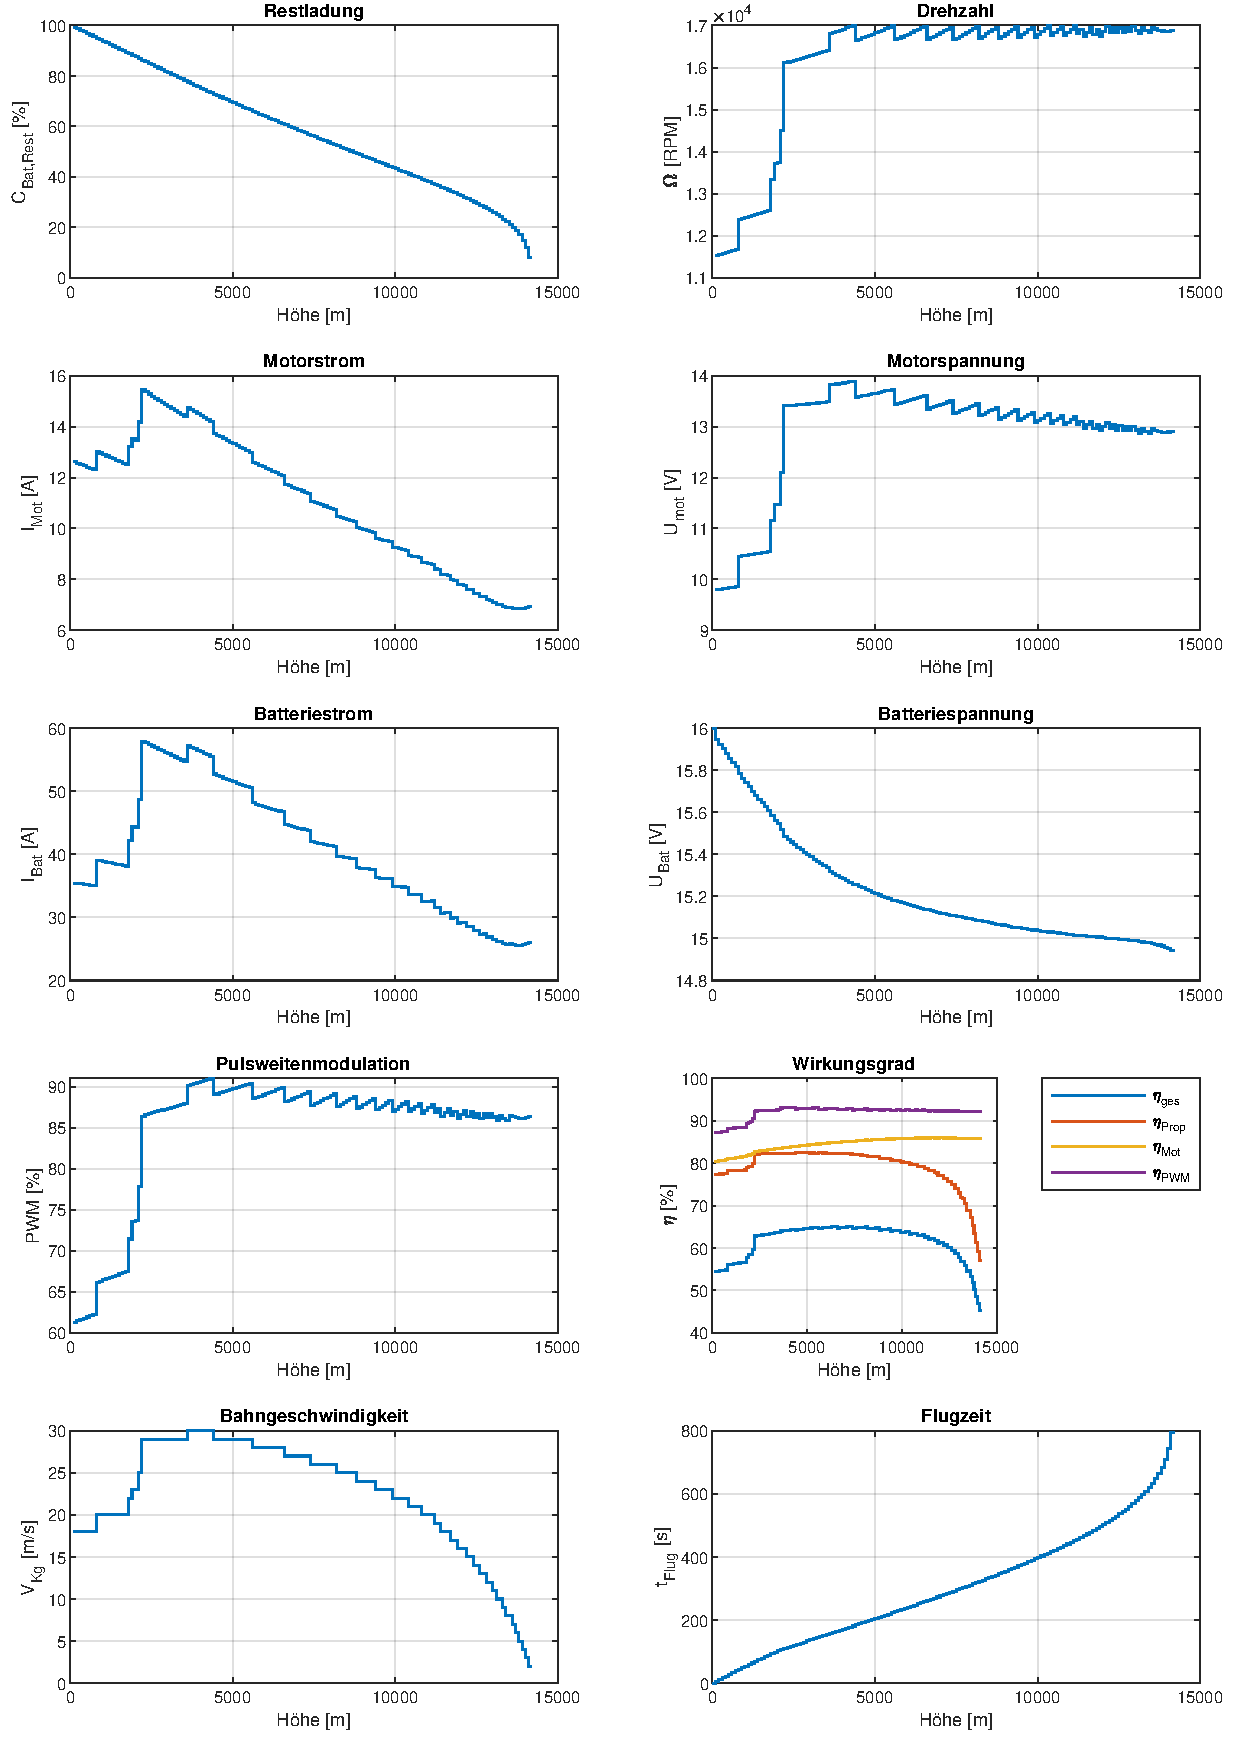
\includegraphics[scale=0.7]{Diagramme/Russland_vvar.pdf}
	\caption{Flugleistungen des Quadrocopter aus \cite{Anderson.2018} mit variabler Steiggeschwindigkeit}
	\label{abb:fp}
\end{figure}


\subsection{Einfluss des Widerstands}
\label{subsec:widerstandseinfluss}
Der Widerstandsbeiwert hat einen entscheidenden Einfluss auf die maximale Steiggeschwindigkeit. Bei einem großen maximalen Motorstrom gilt, dass die Begrenzung der Geschwindigkeit durch den Widerstandsbeiwert erfolgt. Eine sehr hohe Geschwindigkeit verringert zum einen die Flugzeit für einen Höhenbereich, erhöht auf der anderen Seite jedoch den Widerstand und damit zusätzlich die benötigte Leistung. Je geringer der \ensuremath{C_W} gewählt wird, desto höher ist die optimale Steiggeschwindigkeit. Erhöht sich im Umkehrschluss der Luftwiderstand so sinkt die Steiggeschwindigkeit, da der Widerstand mit der Geschwindigkeit quadratisch (Vgl. Gleichung \ref{eq:widerstand}) ansteigt. Im Sinne einer großen maximalen Höhe ist daher eine aerodynamisch günstige Verkleidung des Multicopters anzustreben.
  
\begin{figure}[H]
\centering
	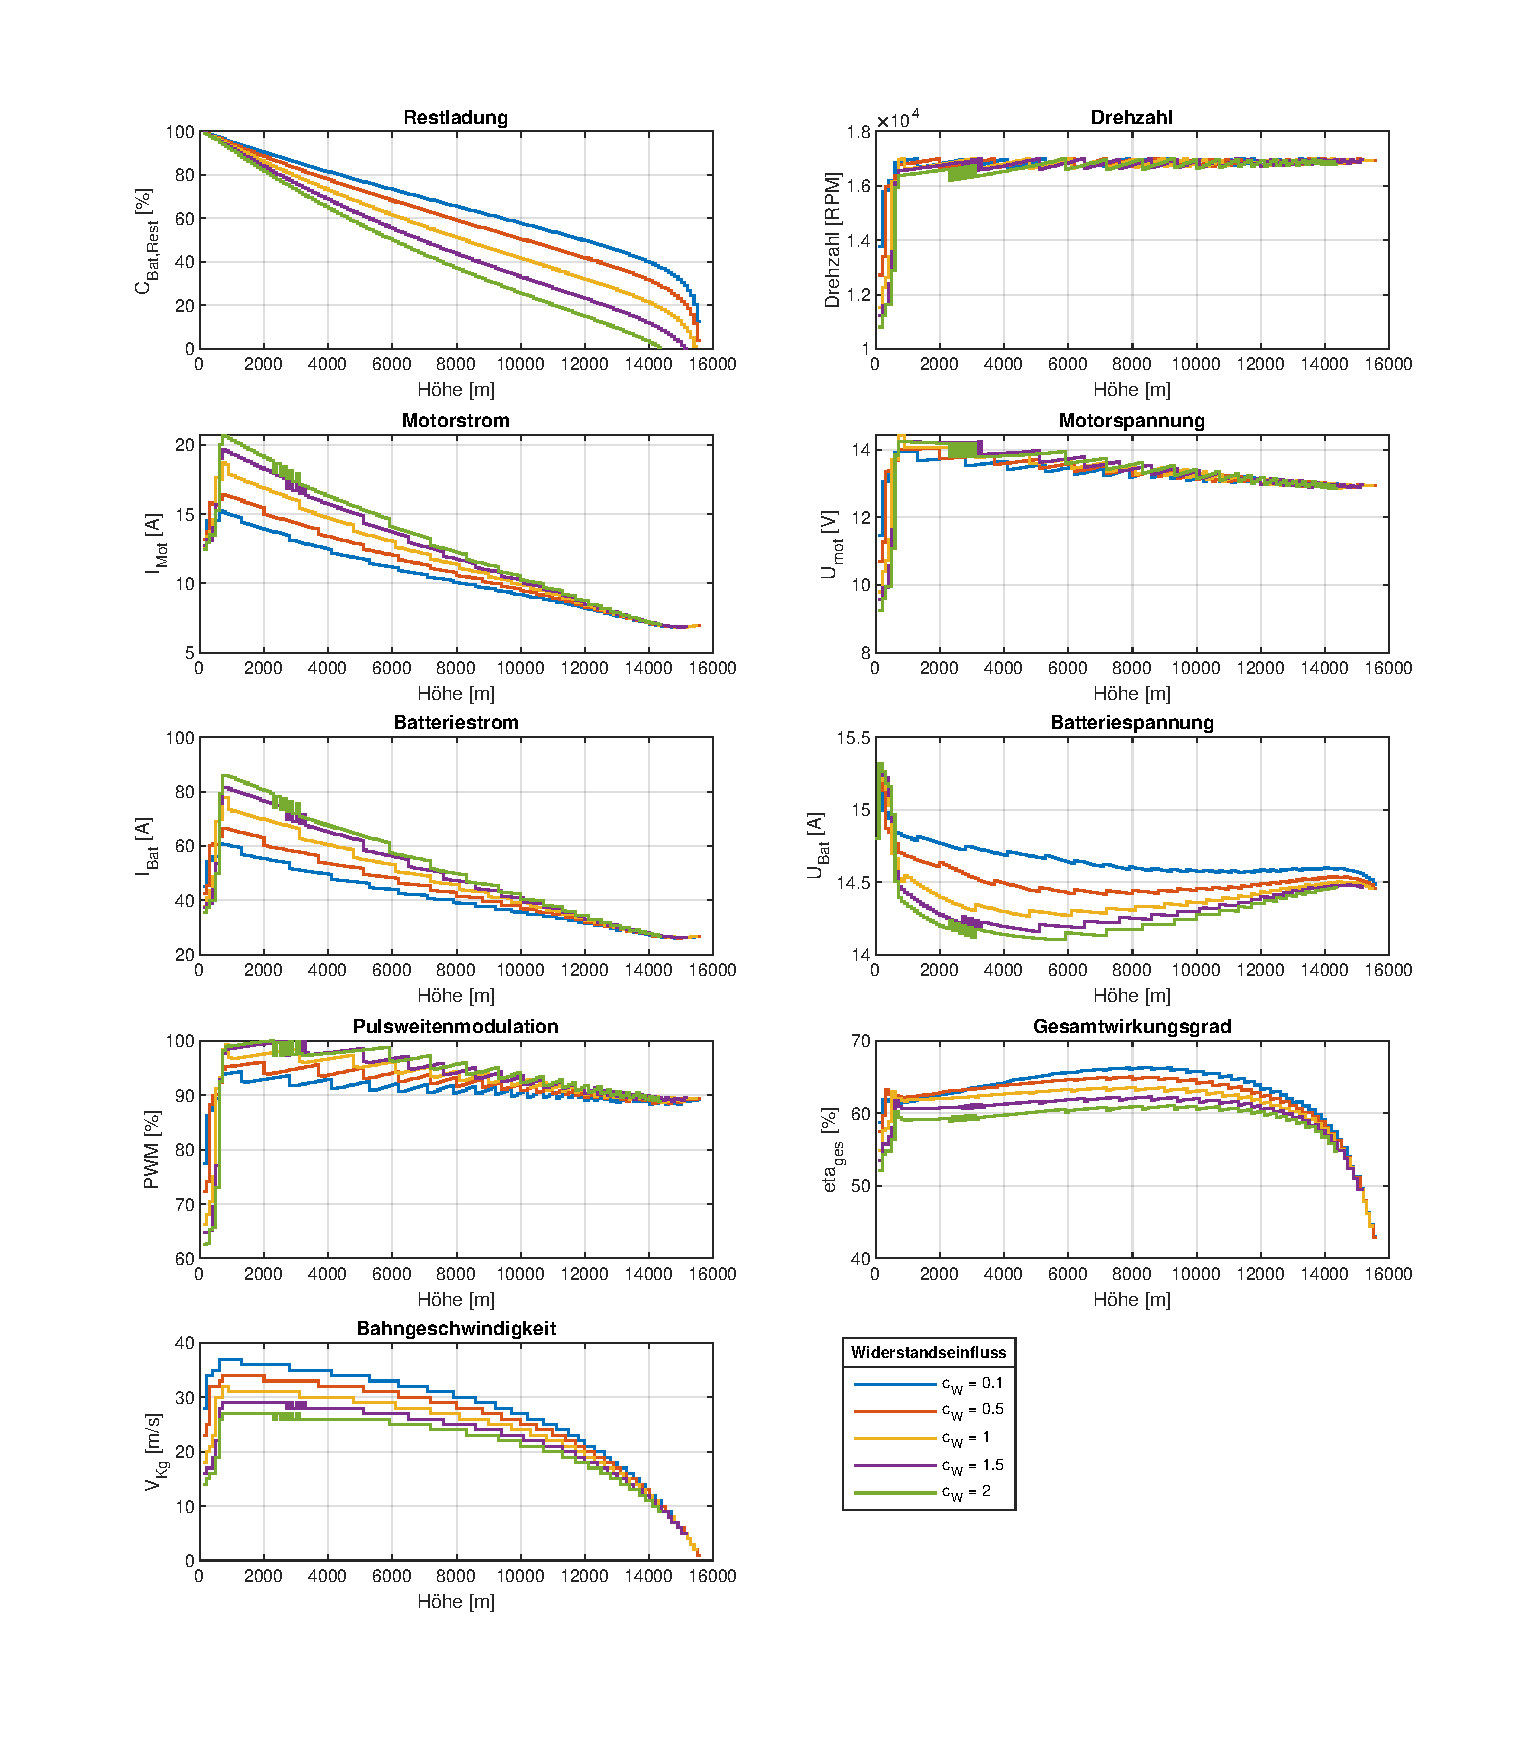
\includegraphics[scale=0.7]{Diagramme/C_W_Untersuchung.pdf}
	\caption{Widerstandseinfluss auf die maximale erreichbare Höhe}
	\label{abb:c_W_einfluss}
\end{figure}

%\begin{itemize}
%	\item der Widerstandsbeiwert hat einen entscheidenden Einfluss auf die maximale Steiggeschwindigkeit
%	\item prinzipiell gilt bei einem großen maximalen Motorstrom, dass die Begrenzung der Geschwindigkeit durch den Widerstandsbeiwert erfolgt. Eine sehr hohe Geschwindigkeit verringert zum einen die Flugzeit für einen Höhenbereich, erhöht auf der anderen Seite jedoch den Widerstand und damit die benötigte Leistung. 
%	\item je geringer der \ensuremath{C_W} gewählt wird, desto höher die Steiggeschwindigkeit, da der Widerstand bei großen Werten noch einen geringen Einfluss hat
%	\item Eine Erhöhung von diesem bezweckt eine Erhöhung eine Verringerung der optimalen Fluggeschwindigkeit
%	\item auch hier gilt wieder, dass der Flug mit \SI{100}{\%} am effizientesten ist
%\end{itemize}

\subsection{Einfluss der Anzahl der Batteriezellen}
Ein weiterer begrenzender Parameter ist die PWM. Die Motorspannung an sich kann nicht beeinflusst werden. Jedoch lässt sich Einfluss auf die Höhe der Motorspannung durch eine Erhöhung der in Reihe geschalteten Batteriezellen nehmen. Mit jeder zusätzlichen Zelle erhöht sich die Batteriespannung um \SI{3,7}{V}. Damit stellt die PWM nicht mehr die Grenze für die Steiggeschwindigkeit dar. Der effizienteste Flugzustand ist nun der bei maximalen, dauerhaften Motorstrom. Jedoch verringert eine höhere Batteriekapazität. Bei gleicher Energiemenge 
\begin{equation}
	E_{Bat} = C_{Bat}\cdot U_{Bat}
\end{equation}
führt eine Erhöhung der Spannung in dem Produkt aus Spannung und Kapazität (\ensuremath{C_{Bat} = I_{Bat}\cdot t_{Flug}}) unweigerlich zu einer Verringerung der Kapazität. Die schlägt sich wieder auf den Kostenfaktor aus, der erreichbaren Flughöhe. Diese Maßnahme ist also mit Bedacht zu wählen. Eine extreme Erhöhung der Zellenanzahl bewirkt außerdem wieder ein Flug mit maximalen Motorstrom.
In Bezug auf die Restladung, Drehzahl, den Motorstrom, Motorspannung und der Bahngeschwindigkeit sind bis auf eine Batteriezellenanzahl von 2 keine großen Unterschiede zu vermerken. Mit der erhöhten Batteriespannung sinkt entsprechend auch die PWM. Zusätzlich verringert sich der Gesamtwirkungsgrad mit der Zellenanzahl. Der Grund hierfür liegt im Wirkungsgrad des Motorreglers. Ein sinkende PWM erhöht die Verluste und verringert den Wirkungsgrad (Vgl. Gleichung \ref{eq:eta_pwm}). Daher sollte der Wirkungsgrad 
%Die Zellen, aus denen eine Batterie besteht, sind meist \textcolor{red}{Massenprodukte} und daher nur in festen Größen und Kapazitäten vorhanden. Erhöht sich nun die Anzahl der Zellen, in diesem Fall wird einfach eine Zelle ergänzt, so erhöht sich auch die Batteriemasse mit der Zelle. Dahingehend ist eine Batteriezellenanzahlerhöhung gegenüber einer Massenerhöhung abzuwägen.

\begin{figure}[H]
\centering
	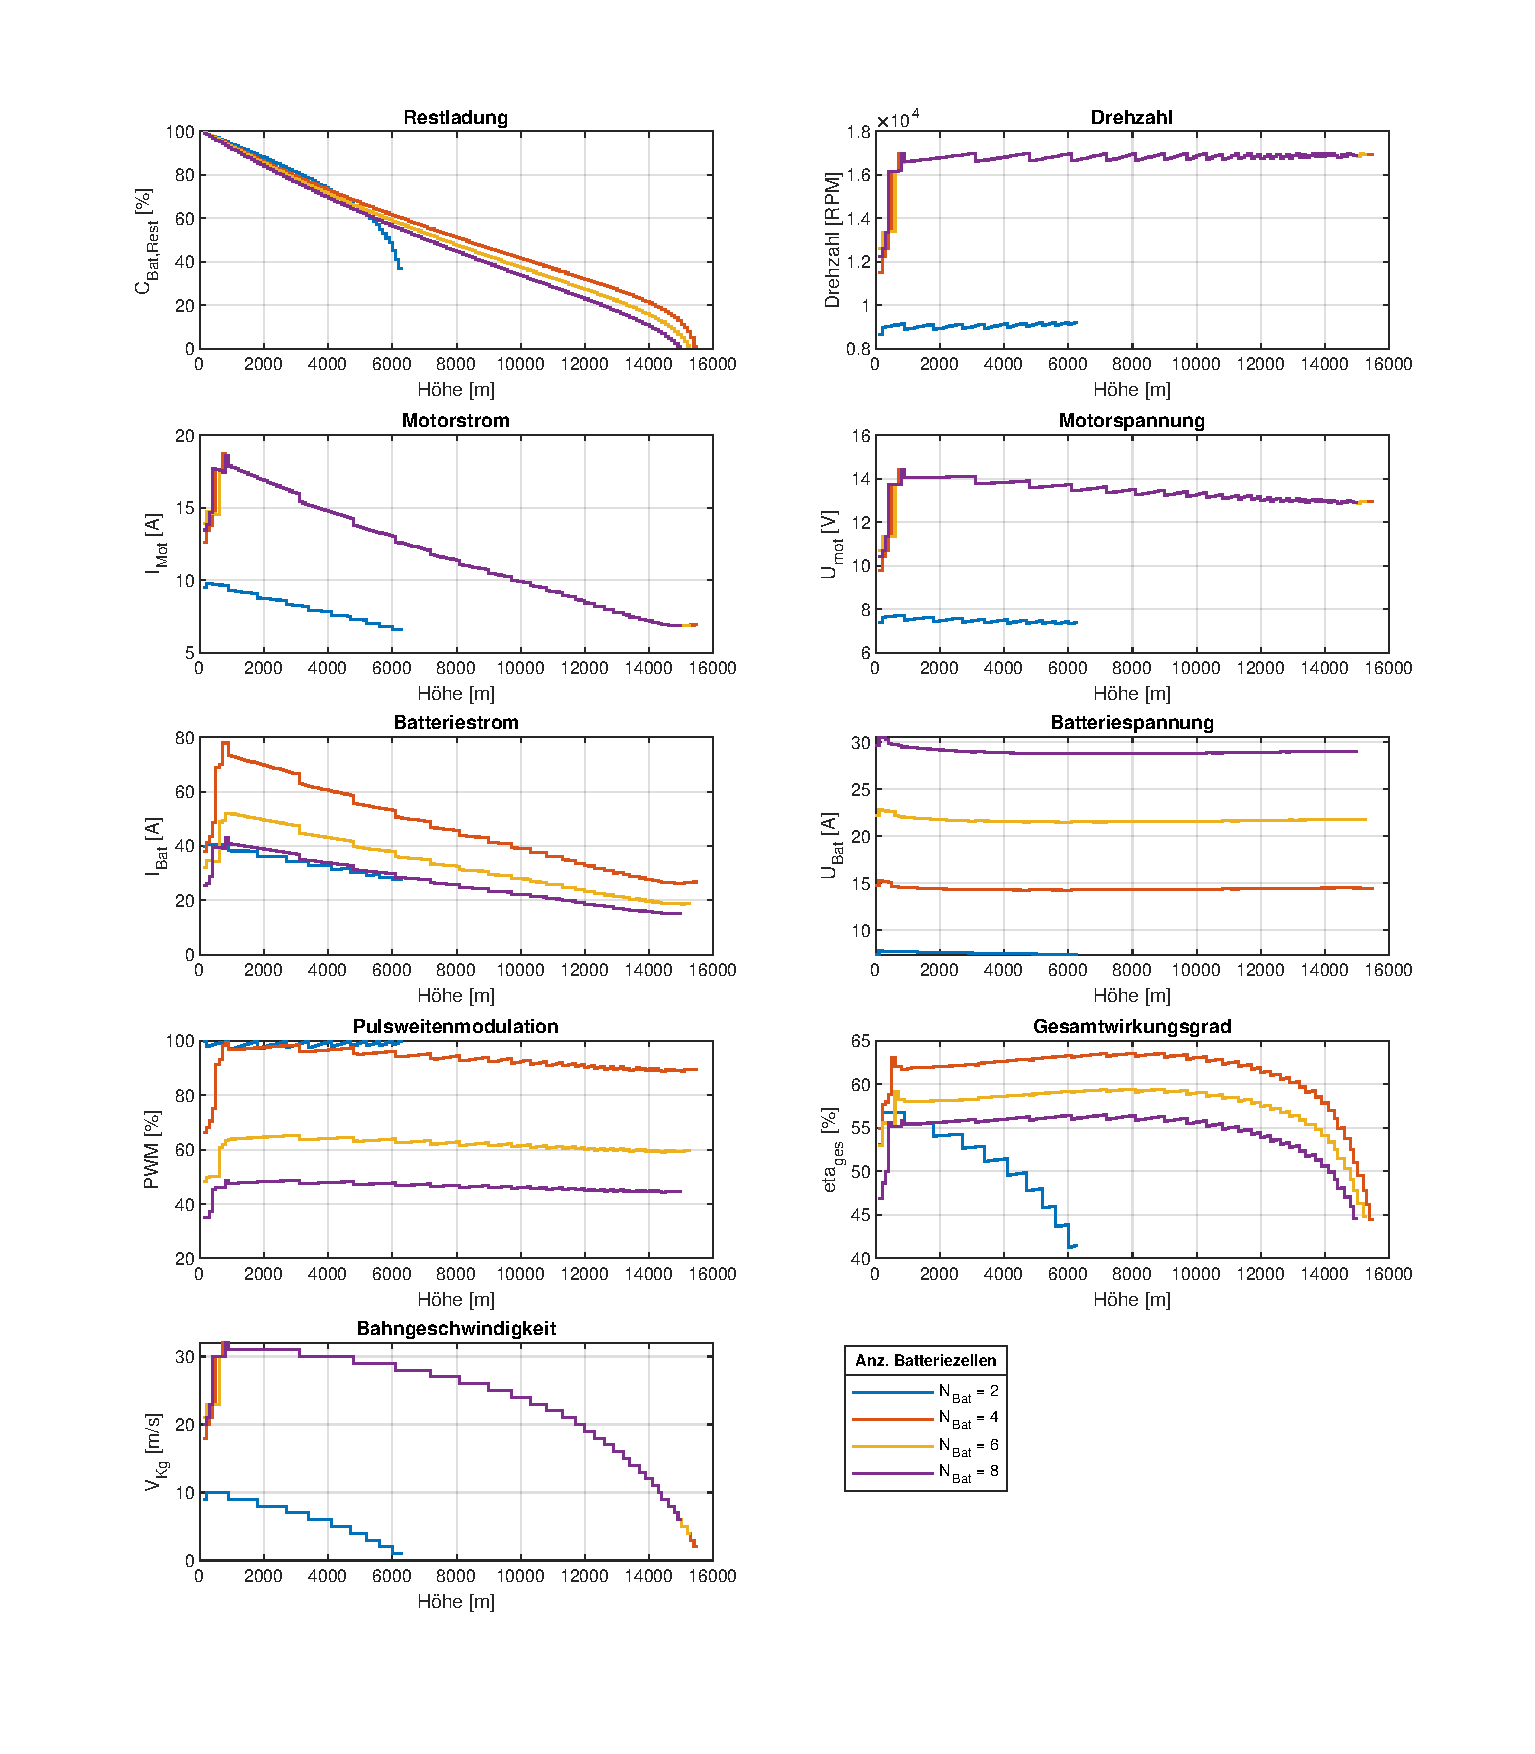
\includegraphics[scale=0.70]{Diagramme/Untersuchung_N_Bat.pdf}
	\caption{Einfluss der Batteriezellenanzahl auf die maximale erreichbare Höhe}
	\label{abb:N_Bat_einfluss}
\end{figure}

\subsubsection{Bedeutung des Reglerwirkungsgrades}
Hinzu kommt, dass bei einer Batterie mit vielen Zellen die PWM bedeutend geringere Werte annimmt als dies bei wenigen Zellen der Fall ist. Der Grund ist die bedeutend höhere Spannung, die mit jeder Zelle um \SI{3,7}{V} steigt. Der Regler muss bei einer gleichen Motorspannung die Batteriespannung stärker modulieren womit auch die Verluste steigen. Der Wirkungsgrad sinkt und damit steigt auch die entnommene Kapazität der Batterie.


\begin{itemize}
	\item eine Verringerung der PWM-Verluste hat bei geringen Anzahl an Batteriezellen keinen Einfluss auf die Flugleistungen
	\item hier ist die PWM sehr schnell auf \SI{100}{\%} wobei sich die Verluste damit minimieren
	\item bei mehr Zellen kann der Einfluss bereits \SI{1000}{m} ausmachen
	\item auch die Kapazität liegt im Durchschnitt höher 
\end{itemize}
%\begin{itemize}
%	\item Einfluss der Batteriezellenanzahl
%	\item als begrenzender Parameter erweist sich die PWM
%	\item dieser kann ausgewichen werden, wenn die Anzahl der Zellen erhöht wird, weil damit die Batteriespannung steigt. 
%	\item damit begrenzt nicht mehr die PWM die Höhe, sondern es sind andere Parameter
%	\item Wenn sie nicht mehr begrenzt, wird als erstes die maximale Motorspannung erreicht und konstant mir ihr geflogen
%	\item dies ist nicht so effizient, wie mit maximaler Leistung, entsprechend verringert sich die max. erreichbare Höhe
%	\item Der Batteriezellenanzahlerhöhung sind Grenzen gesetzt
%	\item Durch eine Erhöhung der Batteriespannung verringert sich um Umkehrschluss die Kapazität der Batterie, da gilt \ensuremath{Wh = Ah\cdot U}
%	\item Eine extreme Erhöhung der Zellenanzahl bewirkt außerdem wieder ein Flug mit maximalen Motorstrom
%\end{itemize}

\subsection{Einfluss des maximalen Motorstroms}
Die Ergebnisse zeigen, dass ein geringer maximaler Motorstrom ebenfalls die Steiggeschwindigkeit begrenzt. Dieser begrenzt die dem Motor entnommene Leistung. 
Folglich ist ein Motor für einen solchen Steigflug zu wählen, der einerseits einen hohen \ensuremath{K_V}-Wert besitzt, andererseits aber auch einen hohen maximalen Dauerstrom besitzt (Vgl. Kap. \ref{subsubsec:mot_prop_kombi}). Ein gutes Beispiel ist der Motor aus Kapitel \ref{chap:nachbildung}.

auch hier \textcolor{red}{KV und KM mit PWM}
Ein hoher KV Wert bedeutet wenig Spannung für viele Umdrehungen allerdings auch einen hohen Strom für das benötigte Drehmoment

%Die Motorleistung
%\begin{itemize}
%	\item Einfluss des maximalen Motorstroms
%	\item ist dieser sehr gering gewählt so stellt er den begrenzenden Parameter
%	\item dieser begrenzt die dem Motor entnommene Leistung 
%	\item entsprechend ist diese groß zu wählen wie beim Cobra-Motor
%\end{itemize}


%******************************************************************

\section{Massenverteilung}
\label{sec:massenverteilung}
Ein weiterer wichtiger Punkt, der an dieser Stelle untersucht werden soll, ist die Massenanteilsverteilung von den Motoren, der Batterie und der Leermasse des Multicopters am Gesamtgewicht. Wiederum stellt der Quadrocopter aus Kapitel \ref{sec:komponenten} die Grundlage der Untersuchung dar. Bei diesem nehmen die Motoren \SI{13,77}{\%}, die Batterie \SI{52,83}{\%} und die der Rahmen mit den übrigen Komponenten \SI{33,4}{\%} der Gesamtmasse von \SI{1060}{g} ein. Für einen Gegenvergleich wird nun ein anderen Quadrocopter mit diesen Massenverhältnissen erstellt. Als Anhaltspunkt dient die Masse der Motoren, da diese durch die Datenbank vollständig definiert sind und eine feste Masse besitzen. Alle anderen Massenverteilungen ergeben sich im Anschluss aus der Motormasse.
Die Massen errechnen sich nach folgendem Schema:
\begin{align}
	m_{ges} &= \frac{n_{Prop}\cdot m_{Mot}}{0.1377} , \\
	m_{Bat} &= m_{ges}\cdot 0.5283 , \\
	m_{copter} &= m_{ges}\cdot 0.334.
\end{align}
Zusätzlich wird jeweils auch die obere Stirnfläche \ensuremath{A_{copter,oben}} mit der Größe angepasst. Im folgenden wird die Masse der Batterie 

\subsection{Ergebnisse}
\newpage
\begin{figure}[H]
%\centering
	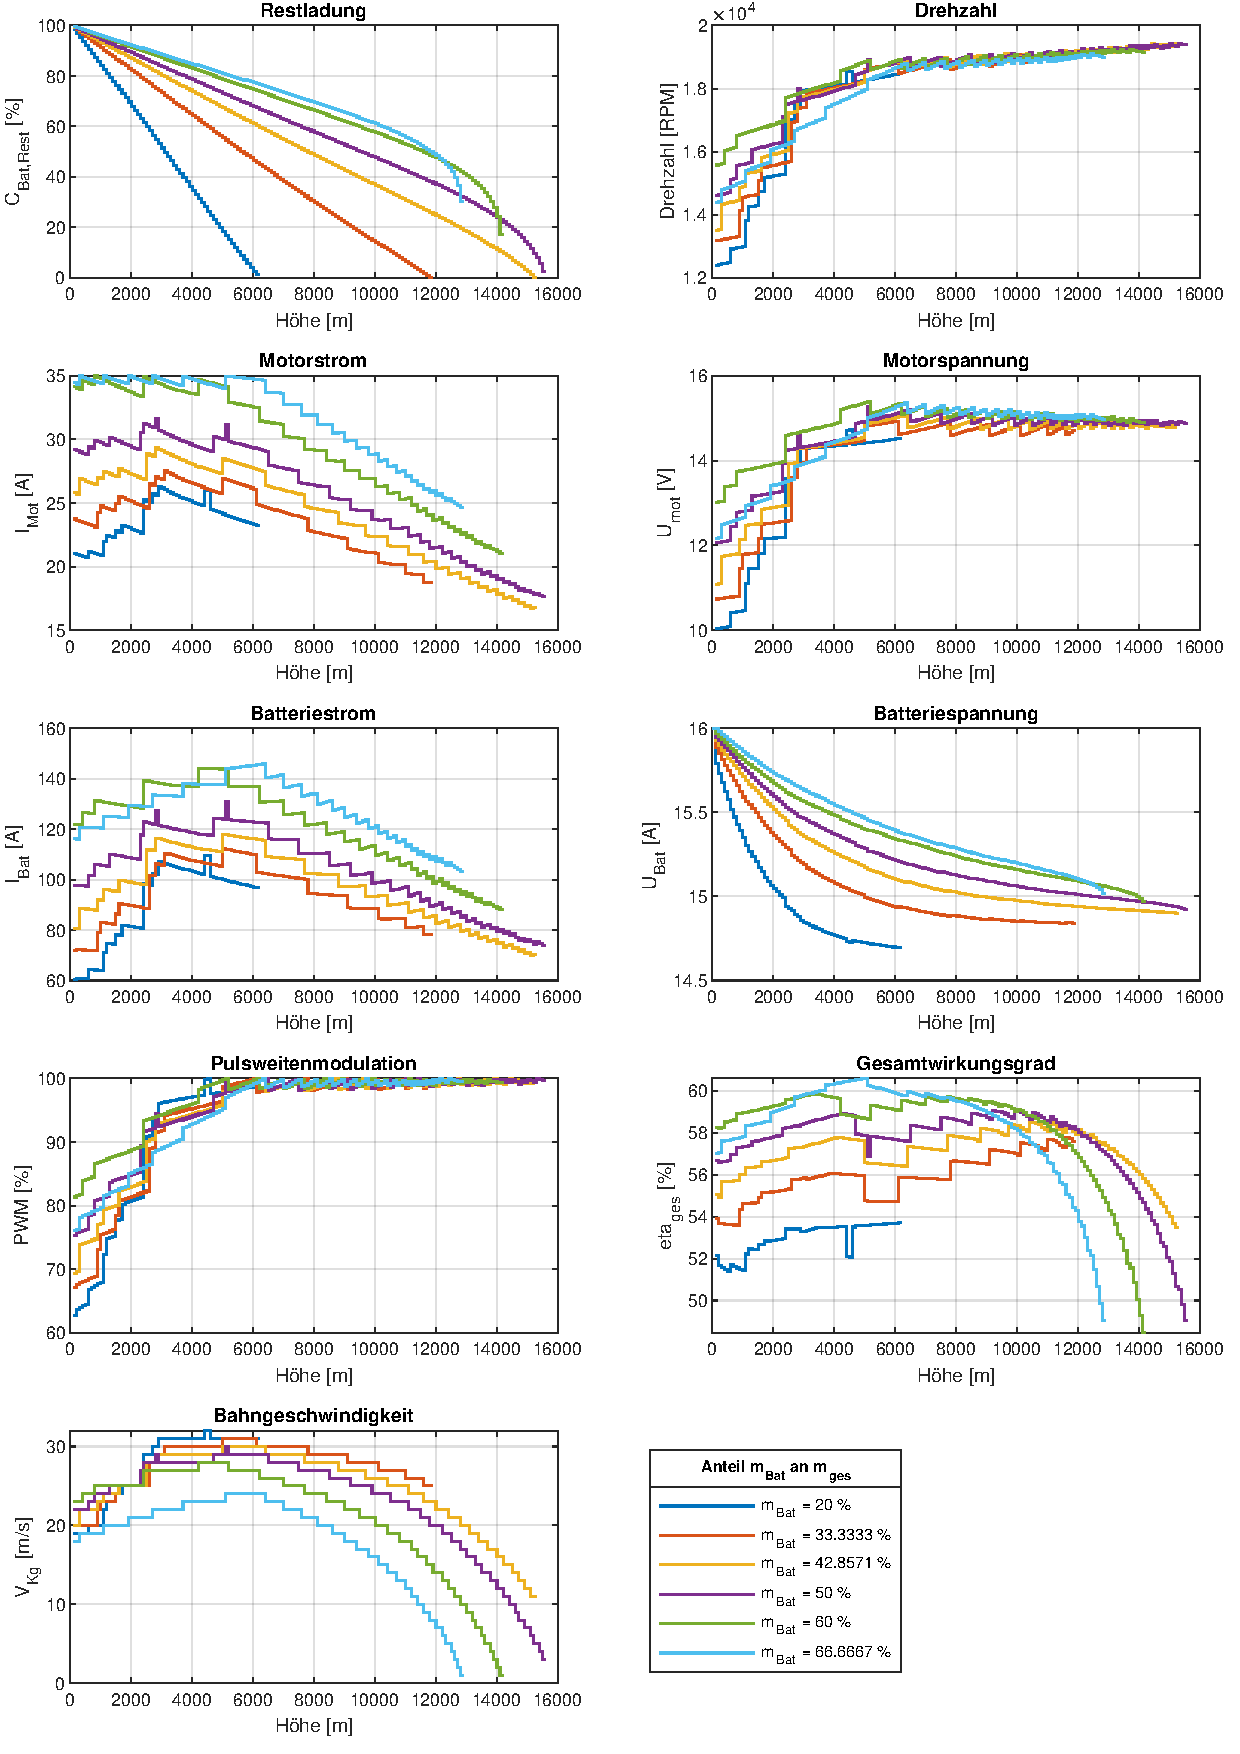
\includegraphics[scale=0.70]{Diagramme/Batteriemasse.pdf}
	\caption{Abhängigkeit der maximalen Höhe von Batteriemasse anteilig an der Gesamtmasse (\ensuremath{m_{Mot}=\SI{106}{g}}, \ensuremath{K_V=\SI{1390}{RPM/V}}, \ensuremath{n_{Prop}=4}, \ensuremath{Propeller=\SI{10x3}{}}, \ensuremath{n_{Bat,cell}=4}, \ensuremath{u_{Wg}=\SI{10}{m/s}})}
	\label{abb:batteriemasse}
\end{figure}

Die Batteriemasse hat einen großen Einfluss auf die Flugleistungen. Die TOC's variieren zwischen eine Spanne von \SI{5000}{m}. Ein Optimum ist bei einer Konstellation erreicht, bei der die Batteriemasse die Hälfte des Gesamtgewichts ausmacht also \SI{50}{\%}. Die Kurven der Restladungskurven von \SI{75}{\%} und \SI{50}{\%} sind bis zu einer Höhe von \SI{12500}{m} deckungsgleich. Danach reduziert sich die Restladung eines Fluggeräts mit einem höheren Anteil der Batteriemasse drastisch. Mit einem zunehmenden Batteriemassenanteil ist für den Steigflug nicht mehr die Kapazität der Batterie begrenzend sondern vielmehr die Leistung und damit die Steiggeschwindigkeit. Mit zunehmender Batteriemasse reduziert sich auch die Steiggeschwindigkeit signifikant. Dies liegt darin begründet, dass die Masse direkt in den Schub mit einfließt (Vgl. Gleichung \ref{eq:neigungswinkel} und \ref{eq:schub_multicopter}). Ein schlechte Verteilung der Massen erhöht somit den Schub und damit die erforderliche Leistung. Dies beeinflusst die Steiggeschwindigkeit, welche die Flugzeit und letztendlich die erreichbare Höhe bestimmt. Weiterhin kann mit größeren Batteriemassen länger mit maximalen Motorstrom geflogen werden, bevor die PWM \SI{100}{\%} erreicht und die Steiggeschwindigkeit sinkt, \textcolor{red}{da das maximale Niveau leistungsbedingt nicht mehr gehalten werden kann.} Für kleinere Batteriemassen beginnt der Flugabschnitt mit \SI{100}{\%} PWM bereits deutlich früher (pro \SI{25}{\%} mehr Batteriemasse sind das ungefähr zusätzliche \SI{2500}{m} Höhe). Dies hat zur Folge, dass die maximale Drehzahl (ca. \SI{18000}{RPM}) früher erreicht ist. Durch die großen Steiggeschwindigkeiten bei kleinen Batteriemassen ist auch ein deutlich stärkerer Einbruch der Batteriespannung zu verzeichnen (ca.\SI{2,5}{V} bei \SI{25}{\%} und nur \SI{1,5}{V} bei größeren Massenanteilen). Zudem ist analog zu den Kurven der Restladung bei den optimalen Konstellationen auch der optimale Gesamtwirkungsgrad erreicht. Die optimale Batteriemasse liegt zwischen \SI{50}{\%} und \SI{52.5}{\%} (Vgl. Anhang).
Dies widerspricht den Aussagen von \cite{Neitzke.2013}, worin die besten Flugleistungen und insbesondere die längste Flugdauer mit einem Anteil der Batteriemasse an der Gesamtmasse von 2/3 angegeben wird. Ein möglicher Grunde sind die unterschiedlichen Flugzustände. Neitzke hat seine Untersuchungen ausschließlich im Hovern gemacht. Somit fehlt in seinen Betrachtungen der Höheneinfluss und der Einfluss einer Steiggeschwindigkeit. \textcolor{red}{Neitzke nimmt einen konstanten Wirkungsgrad für alle an, was aber nicht für alle Flugzustände gilt.}\\
Zusammengenommen weisen die obige Untersuchung der Massenverteilung und der Quadrocopter aus Russland das gleiche Ergebnis auf. Die Konstellation des Quadrocopters aus \cite{Anderson.2018} erweist sich bereits in diesem Sinne als optimal.\\
Es ist außerdem ersichtlich, dass die Flugleistung und -dauer noch weiter verbessert werden können, wenn der Massenanteil des Rahmens und aller übriger kleiner wird und die Masse der Batterie im Gegensatz steigt, i.e. eine Tendenz der Coptermasse gegen Null (\ensuremath{m_{Copter}\rightarrow 0} und \ensuremath{m_{Bat}\rightarrow (m_{Bat}+m_{Copter})})


%******************************************************************

\section{Größe und Anzahl der Propeller des Fluggerätes}
\label{sec:groesse}
Ein weitere Einfluss auf die Flugleistungen stellt das Gesamtgewicht des Fluggerätes dar. Dabei wird das Fluggerät äquivalent, das heißt die Massenverhältnisse von Motoren, Batterien und die Leermasse bleiben im Verhältnis zum Gesamtgewicht konstant. Das Verhältnis orientiert sich an der Massenverteilung aus Kapitel \ref{sec:massenverteilung}. Dieses Verhältnis wird für jede Größenskalierung gewahrt. Als Anhaltspunkt dient die Masse der Motoren, da mit diese durch die Datenbank vollständig definiert sind und eine feste Masse besitzen. Die Propellerauswahl findet nach den Herstellerempfehlungen statt. Alle anderen Massenverteilungen ergeben sich im Anschluss aus der Motormasse analog zu Kapitel \ref{sec:massenverteilung}.

\subsection{Ergebnisse}
\label{subsec:ergebnisse_groesse}

\begin{figure}[H]
%\centering
	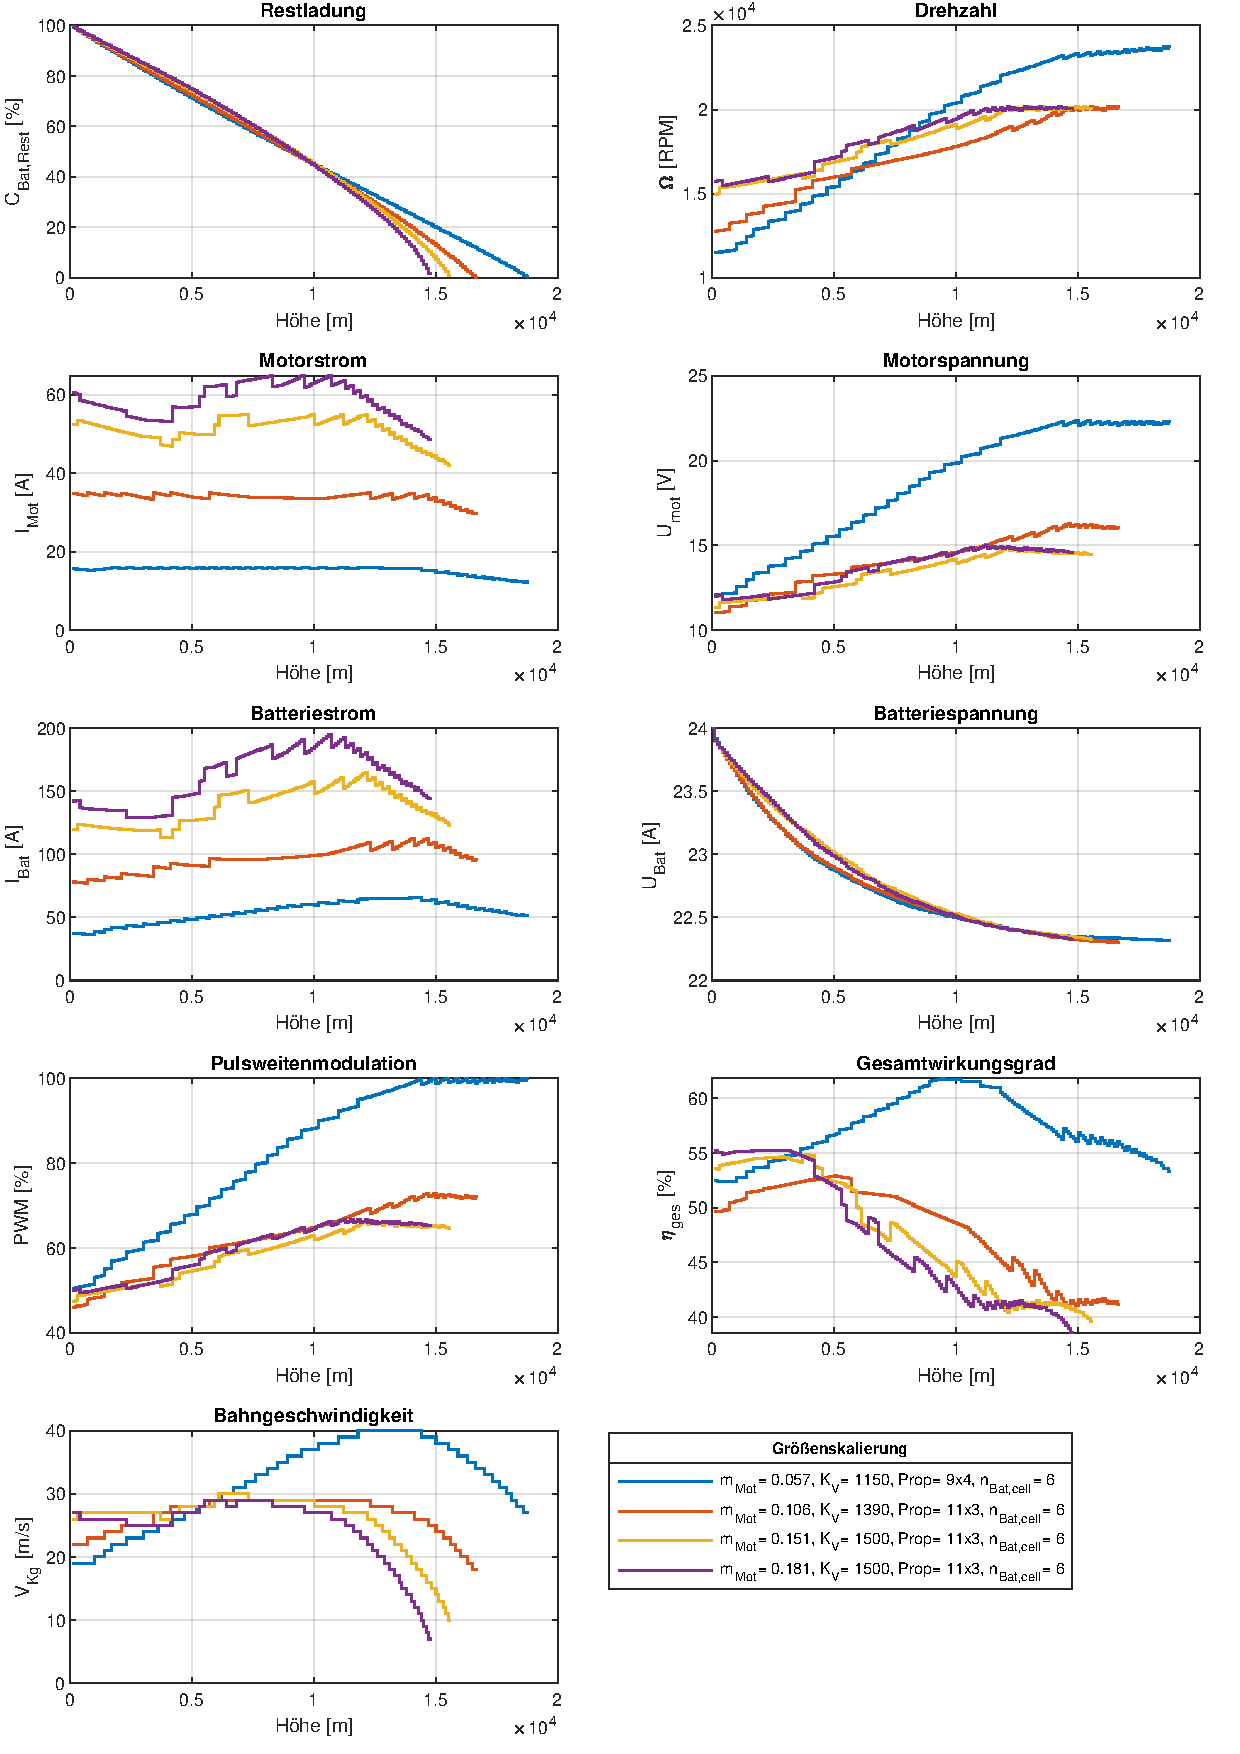
\includegraphics[scale=0.7]{Diagramme/Groessenskalierung.pdf}
	\caption{Einfluss der Größenveränderung auf die maximal erreichbare Höhe}
	\label{abb:groessenskalierung}
\end{figure}
Eine äquivalente Größenskalierung besitzt einen vernachlässigbar kleinen Einfluss auf die Kostenfunktion, die maximale Höhe (Vgl. Abb. \ref{abb:groessenskalierung}). 
\textcolor{red}{Begründung für Reichweitenunabhängigkeit von der Flugmasse}. An dieser Stelle kann somit festgehalten werden, dass eine Größenskalierung keinen Einfluss auf die Flugleistungen hat. Die Vorteile eine größeren Masse liegen für reale Anwendungsfälle vorrangig in der Massenträgheit. In einem Höhensektor von \SI{0}{} bis \SI{15000}{m} treten im Durchschnitt starken Winde mit \SI{100}{km/h} auf. Die Einflüsse von Böen in diesen Größenordnungen auf einen Multicopter fällt geringer aus, wenn die Masse höher. Dies erfordert im Umkehrschluss weniger Energie zur Kurs- und Lagekorrektur.

\begin{itemize}
	\item größter Einfluss ist bei bei Motor zu verzeichnen. größerer maximaler Motorstrom
	\item Die Drehzahl hängt auch sehr vom Motorab. genereller Trend geht in richtung einer größeren Drehzahl bei größeren Motoren und mit höherem \ensuremath{K_V}-Wert
	\item entsprechend sinkt auch die Motorspannung mit dem \ensuremath{K_V}-Wert und \SI{100}{\%} PWM wird später erreicht. außerdem sinkt die optimale Steiggeschwindigkeit mit dem Gewicht des Gewicht
	\item der Gesamtwirkungsgrad ist bei einem geringen Gewicht deutlich höher und das schlägt sich auch auf die Restladung aus
	\item bei geringerem Gewicht begrenzt die mögliche Steiggeschwindigkeit den Flug, bei höherem Gewicht ist es die Restladung 
\end{itemize}

\subsection{Anzahl der Propeller}
Wie sich oben zeigte, hat eine uniforme Skalierung des Fluggerätes keinen Einfluss auf dessen Flugleistung. Bisher wurde dabei nur Fluggeräte mit vier Rotoren untersucht. Dabei gilt es noch die Abhängigkeit der Flugleistungen von der Rotoranzahl zu überprüfen. 

\subsection{Ergebnisse}
\begin{figure}[H]
%\centering
	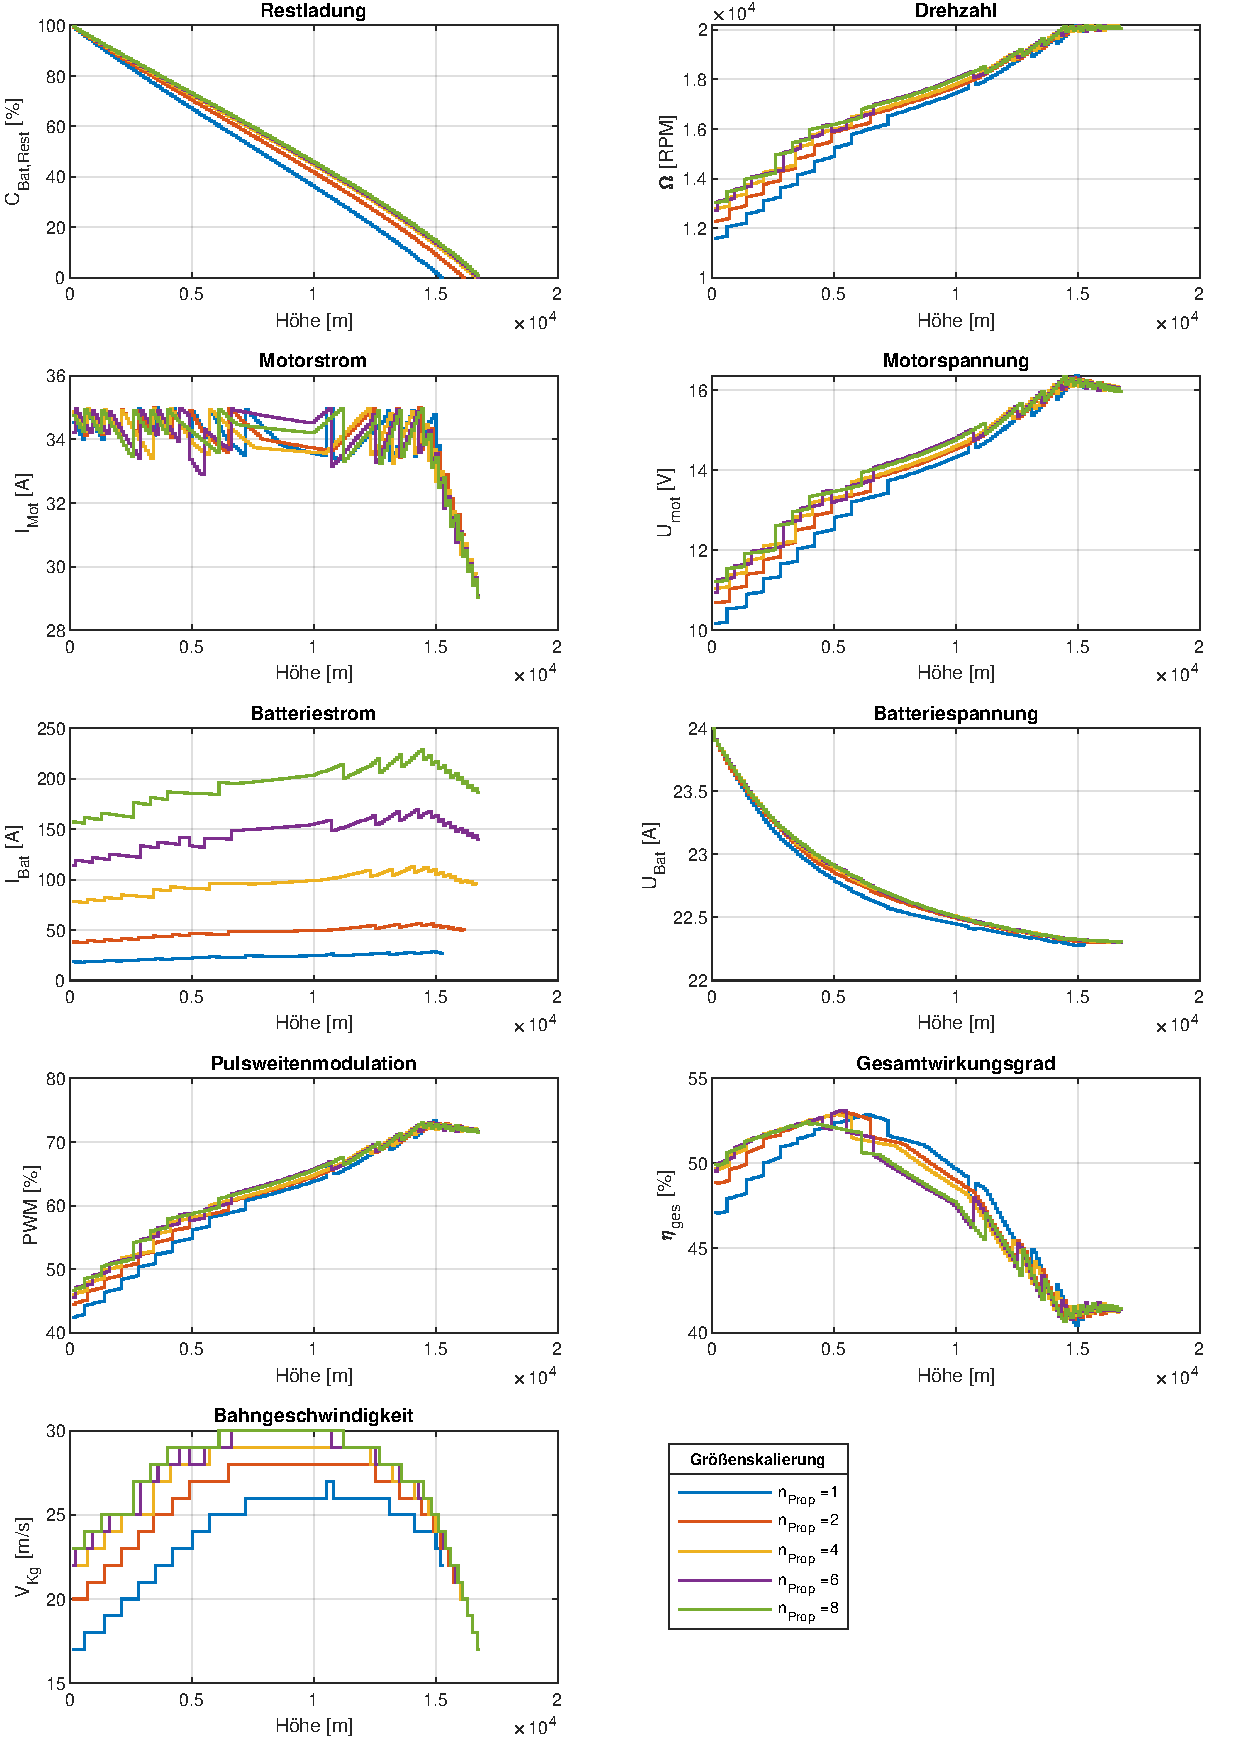
\includegraphics[scale=0.7]{Diagramme/Anz_Prop.pdf}
	\caption{Einfluss der Propelleranzahl auf die maximal erreichbare Höhe (\ensuremath{m_{Mot}=\SI{106}{g}}, \ensuremath{K_V=\SI{1390}{RPM/V}}, \ensuremath{n_{Prop}=4}, \ensuremath{Propeller=\SI{10x3}{}}, \ensuremath{n_{Bat,cell}=4}, \ensuremath{u_{Wg}=\SI{10}{m/s}})}
	\label{abb:groessenskalierung}
\end{figure}
Analog zu den obigen Ergebnissen bewirkt eine äquivalente Veränderung der Rotoranzahl keine nennenswerten Änderungen der maximalen Flughöhe für gleiche Motoren. Die Begründung ist dieselbe wie Kapitel \ref{subsec:ergebnisse_groesse}. An dieser Stelle sind jedoch Einschränkungen vorzunehmen. 
Der Monocopter erreicht die gleiche maximale Höhe wie die anderen Konstellationen. Der Monocopter benötigt jedoch zusätzlich noch Aktuatorik für die Abdeckung aller vier Stellgrößen, sprich den 3 rotatorischen (Rollen, Nicken und Gieren) und einem translatorischen. Weiterhin muss ein Drehmomentenausgleich vollzogen werden, sei es durch einen Heckrotor, eine angepasste Steuerung, die Formgebung des Rumpfes oder durch sonstige Mechanismen.
Diese zusätzliche Aktuatorik benötigt der Duocopter ebenfalls. Ein Drehmomentenausgleich ist hier jedoch nicht notwendig.
Beide erwähnten Punkte erhöhen die Gesamtmasse und benötigen zusätzlich Energie. Dies verringert die Gesamthöhe. 
Für mehrere Propeller müssten noch Penaltyfaktoren mit berücksichtigt werden, da mit der Anzahl der Propeller auch die Struktur und dessen Gewicht zunimmt. 

%\begin{itemize}
%	\item wenn eine äquivalente Veränderung der Konstellation vorgenommen wird, sind die Ergebnisse beinahe identisch, es ergeben sich keine Leistungsunterschiede
%	\item der Duocopter erreicht beinahe ebenso hohe, wenn nicht sogar bessere Werte als die Multicopter
 %	\item allerdings müssen die Ergebnisse unter realistischen Gesichtspuntken betrachtet werden
%	\item Für den Monocopter fehlt die Berücksichtigung der Drehmomentausgleichenden Mechanismen, sei es ein Hekcrotor oder ähnliches
%	\item diese benötigen auch Leistung aus der Batterie und verschlechtern die bisher erbrachten Flugleistungen deutlich
	%\item ein Duocopter scheint eine gute Alternative zu sein, allerdings ist sein Flugverhalten eher nachteilig
%	\item langsame Reaktionszeiten, ein träges Reaktionsverhalten, komplizierte Regelung, wird leicht instabil und besitzt eine komplizierte Technik
%	\item für mehrere Propeller müssten noch Penaltyfaktoren mit berücksichtigt werden, da mit der Anzahl der Propeller auch die Struktur und dessen Gewicht zunimmt
%	\item somit stellt der Quadrocopter die beste Lösung dar
%\end{itemize}


\section{Verstellpropeller}
\label{sec:verstellprop}
Ein bisherige Begrenzung der Flugleistungen erfolgte häufig durch die maximale Drehzahl des Propellers, die indirekt die Motorspannung beeinflusst. 
Besonders auffällig bei vorherigen Untersuchungen (vor allem in Bezug auf die Untersuchungen des Quadrocopters aus Kap. \ref{chap:nachbildung})  ist, dass bei Propeller mit einem geringen Pitch die Drehzahl deutlich schneller steigt, als bei einem Propeller mit einem großen Pitch. Da vor allem die Drehzahl die Motorspannung bestimmt, ist eine Verringerung der Drehzahl bei gleichem Schub von Interesse / anzustreben. Mit zunehmender Flughöhe verringert sich die Dichte und damit auch der Schub, wenn die Rotordrehzahl oder der Blattanstellwinkel konstant gehalten werden. Diesem kann mit einer Erhöhung der Drehzahl oder mit einer Erhöhung der Blattanstellwinkel ausgeglichen werden. Während bei einem Drehflügler mit Flugtriebwerk nur eine Blattverstellung, nicht aber eine Drehzahlerveränderung möglich ist, besitzen elektrisch, propellergetriebene Fluggeräte beide Möglichkeiten. Dies kann mit einem Verstellpropeller und entsprechender Aktuatorik realisiert werden. \\
Im Rahmen dieser Untersuchung liegen nur Propellerkennfelder mit einem konstanten Pitch vor. Das Vorgehen für einen Propeller mit variablem Pitch sieht so aus, dass für einen vorgegebenen Durchmesser alle Kennfelder mit diesem Durchmesser der Datenbank entnommen werden. Danach wird in der Leistungsuntersuchung jeder Propeller mit unterschiedlichem Pitch, aber gleichem Durchmesser, gegeinander abgewogen. Die Auswahl für den in dem betrachteten Flugmoment besten Pitch erfolgt wieder über die Energiebetrachtung, analog zum Steigwinkel und der Steiggeschwindigkeit.
%	\item analog steigt \textcolor{red}{van der Wall, diagramm mit theta nachgucken} bei konstanter Drehzahl (Vgl. z.B. Hubschrauber) der Pitch, sprich Theta mit einem größer werdendem Schubbeiwert und damit auch mit der Höhe. 
%	\item bei einem elektrisch propellergetriebenen Fluggerät können mit einem Mechanismus der Pitch und über den Motor die Drehzahl geändert werden. 
%	\item dies kann im folgenden über die Auswertung der Kennfelder in der APC Datenbank erfolgen, die den gleichen Durchmesser besitzen, aber unterschiedliche feste Pitches
%	\item Die Auswahl für den in dem betrachteten Flugmoment besten Pitch erfolgt wieder über die Energiebetrachtung, analog zum Steigwinkel und der Steiggeschwindigkeit
%	\item Programmablauf in unterer Abbildung
%\end{itemize}

\subsection{Ergebnisse}
\subsection{Ergebnisse}
\begin{figure}[H]
%\centering
	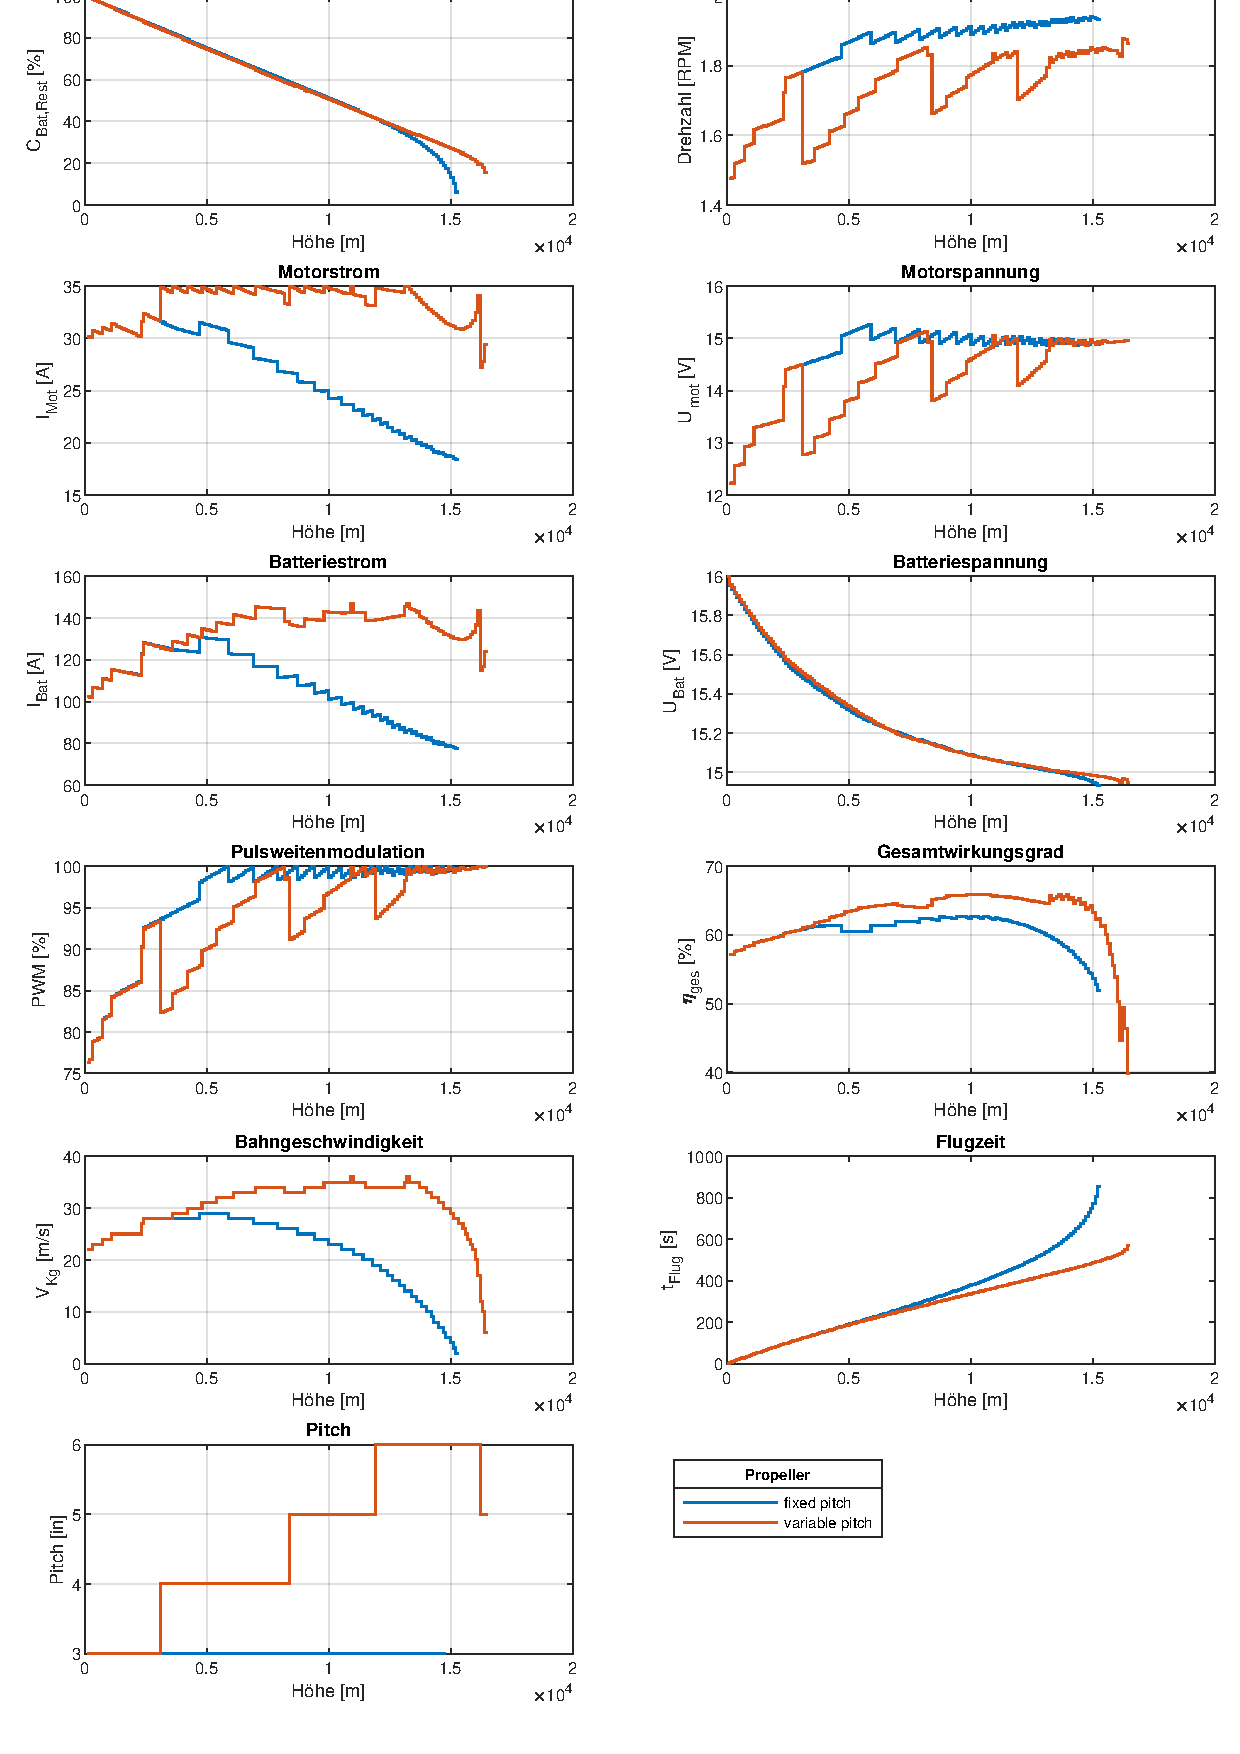
\includegraphics[scale=0.7]{Diagramme/Verstellpropeller.pdf}
	\caption{Verstellpropeller}
	\label{abb:verstellpropeller}
\end{figure}
Der zusätzliche Höhengewinn durch einen Verstellpropeller ist gerade einmal \SI{10000}{m}. Die Leistungsparameter beider Propellerarten sind für die ersten \SI{10000}{m} identisch. Dies liegt am gleichen Pitch. Zuerst ist wieder ein Flug mit maximalen Motorstrom am effizientesten bis die PWM wieder \SI{100}{\%} erreicht und folglich der Motorstrom und der Batteriestrom abfallen. Da die Motorspannung konstant bleibt, bleibt auch die Drehzahl konstant. Die Bahngeschwindigkeit sinkt jedoch kontinuierlich ab. Während sich dieser Zustand beim Propeller mit festem Anstellwinkel nicht ändert, ist ab \SI{10000}{m} Steigflug ein Anstellwinkel von \SI{4}{in} für den Verstellpropeller energetisch effizienter. Dies bewirkt, dass die Drehzahl und damit einhergehend die Motorspannung abfällt, während gleichzeitig der Motorstrom zum zweiten Mal auf sein maximales Niveau steigt. Gleichzeitig steigen auch der Wirkungsgrad und die Bahngeschwindigkeit erneut. Dieser Zustand kann ebenfalls wieder solange gehalten werden bis die PWM \SI{100}{\%} erreicht und somit die Bahngeschwindigkeit bis auf \SI{0}{m/s} absinkt. Damit ist das Ende des Steigflugs erreicht. \\
	Der Vorteil eines Verstellpropellers ist vergleichsweise gering. Dazu müssen auch noch folgende Einschränkungen vorgenommen werden. Der Verstellpropeller kann nur im Rahmen der in der APC-Datenbank vorhanden Propeller modelliert werden. Dies setzt Ungenauigkeiten voraus, da eine kontinuierliche Verstellung nicht nachgebildet werden kann und nur so viele Verstellungen berücksichtigt werden können, wie auch Propeller mit verschiedenen Pitches in der Datenbank vorhanden sind. \textcolor{red}{Zudem ist man auf die Kennfelder angewiesen.}. An dieser Stelle wurde der Propeller in gewisser Weise idealisiert. So wurde unter anderem die verlängerte Blattaufhängung außer Acht gelassen. Dies führt zu zusätzlichen Verlusten an der Blattwurzel und einer Verringerung des effektiven Radius. Bei einem Propeller mit konstantem Anstellwinkel kann diese sehr kurz gehalten werden, weshalb das profilierte Rotorblatt deutlich früher beginnt. Dies ist bei dem hier modellierten Verstellpropeller nicht berücksichtigt worden.\\
Weiterhin wurden in dieser Betrachtung das Gewicht des Verstellmechanismus an sich und der Aktuatorik für jeden einzelnen Propeller nicht berücksichtigt. Weiterhin bedeuten die Aktuatoren zusätzliche Verbraucher, die mitunter deutlich schneller zu einem Flug bei \SI{100}{\%} PWM führen würden. Letztendlich ist der fehlende Schub in großen Höhen nicht das Begrenzungsmerkmal, sondern die Drehzahl des Propellers und Motors sowie die Batteriespannung. Letztere macht den Verstellpropeller ein weiteres Stück redundant (Vgl. \textcolor{red}{Anhang}). Mit einem hohen Batteriestrom verschiebt sich der Bereich, in dem ein größerer Pitch vorteilhafter ist, noch weiter in größere Höhen. Damit sinkt auch die Einsatzdauer und schließlich der Nutzen. 
Schlussendlich bringt der Verstellpropeller einen entscheidenden Vorteil der Autorotation mit, der weniger für den Steigflug als für den anschließenden Sinkflug von Bedeutung ist. Durch die Autorotation ist ein antriebsloser Sinkflug möglich. Damit könnte die Batterie noch weiter entladen werden bevor ein Sinkflug eingeleitet werden muss, was im Umkehrschluss die erreichbare Höhe steigert. 

%\begin{itemize}
%	\item Der Verstellpropeller bringt gerade einmal einen Vorteil von \SI{1000}{m}Höhe.
%	\item Die Leistungsparameter sind für die ersten \SI{10000}{m} identisch. Dies liegt am gleichen Pitch.
%	\item Zuerst ist wieder ein Flug mit maximalen Motorstrom am effizientesten bis die PWM wieder \SI{100}{\%} erreicht und folglich der Motorstrom und der Batteriestrom abfallen. Da die Motorspannung konstant bleibt, bleibt auch die Drehzahl konstant. Die Bahngeschwindigkeit sinkt jedoch kontinuierlich ab.
%	\item Während sich beim fixed pitch Propeller dieser Zustand nicht ändert, kann der variable pitch Propeller der
%	\item ab \SI{10000}{m} ist ein Steigflug mit einem Pitch von \SI{4}{in} effizienter. 
%	\item Dies bewirkt, dass die Drehzahl und damit einhergehend die Motorspannung abfällt, während gleichzeitig der Motorstrom zum zweiten Mal auf sein maximales Niveau steigt. Gleichzeitig steigen auch der Wirkungsgrad und die Bahngeschwindigkeit erneut. Dieser Zustand kann ebenfalls wieder solange gehalten werden bis die PWM \SI{100}{\%} erreicht und somit die Bahngeschwindigkeit bis auf \SI{0}{m/s} absinkt. Damit ist das Ende des Steigflugs erreicht. \\
%	Der Vorteil eines Verstellpropellers ist vergleichsweise gering. Dazu müssen auch noch folgende Einschränkungen vorgenommen werden. Der Verstellpropeller kann nur im Rahmen der in der APC-Datenbank vorhanden Propeller modelliert werden. Dies setzt Ungenauigkeiten voraus, da eine kontinuierliche Verstellung nicht nachgebildet werden kann und nur so viele Verstellungen berücksichtigt werden können, wie auch Propeller mit verschiedenen Pitches in der Datenbank vorhanden sind. \textcolor{red}{Zudem ist man auf die Kennfelder angewiesen.}. An dieser Stelle wurde der Propeller in gewisser Weise idealisiert. So wurde unter anderem die verlängerte Blattaufhängung außer Acht gelassen. Dies führt zu zusätzlichen Verlusten an der Blattwurzel. Bei einem Propeller mit konstantem Anstellwinkel kann diese sehr kurz gehalten werden, weshalb das effektive Blatt bei einem deutlich kleineren Radius anfängt.
	
%Unter anderem wurden in dieser Betrachtung das Gewicht des Verstellmechanismus an sich und der Aktuatorik für jeden einzelnen Propeller nicht berücksichtigt. Weiterhin bedeuten die Aktuatoren zusätzliche Verbraucher, die mitunter deutlich schneller zu einem Flug bei \SI{100}{\%} PWM führen würden. Letztendlich ist der fehlende Schub in großen Höhen nicht das Begrenzungsmerkmal, sondern die Drehzahl des Propellers und Motors sowie die Batteriespannung. Letztere macht den Verstellpropeller ein weiteres Stück redundant (Vgl. \textcolor{red}{Anhang}). Mit einem hohen Batteriestrom verschiebt sich der Bereich, in dem ein größerer Pitch vorteilhafter ist, noch weiter in größere Höhen. Damit sinkt auch die Einsatzdauer und schließlich der Nutzen. 
%Schlussendlich bringt der Verstellpropeller einen entscheidenden Vorteil der Autorotation mit, der weniger für den Steigflug als für den anschließenden Sinkflug von Bedeutung ist. Durch die Autorotation ist ein antriebsloser Sinkflug möglich. Damit könnte die Batterie noch weiter entladen werden bevor ein Sinkflug eingeleitet werden muss, was im Umkehrschluss die erreichbare Höhe steigert. 
%	\item somit ergibt sich keinerlei Vorteil für die Benutzung eines Verstellpropellers
%	\item Trotzdem muss berücksichtigt werden, das der Propeller nur im Rahmen der in der APC-Datenbank vorhanden Propeller modelliert werden kann.
%	\item dies setzt Ungenauigkeiten voraus, da eine kontinuierliche Verstellung nicht nachgebildet werden kann und nur so viele Verstellungen berücksichtigt werden können, wie auch in der Datenbank vorhanden sind
%	\item außerdem ist man auf die Kennfelder angewiesen
%	\item kann aber für den Sinkflug bedeutend sein, weil mit der Verstellung die Autorotation ermöglicht wird
%\end{itemize}


\section{Stufenloses Getriebe}
\label{sec:getriebe}
Eine häufige Begrenzung der Leistung ist die maximale Drehzahl des Motors oder des Propellers. Diese nimmt mit großen Höhen stark zu. Ein stufenlos verstellbares Getriebe bringt Vorteile in der Begrenzung der maximalen Drehzahl (Machzahleffekte, Strömungsablösung etc.), dass heißt durch den Einsatz eines Getriebes kann die Drehzahl für den Motor entsprechend angepasst werden, sodass diese nicht mehr den Flaschenhals für einen Steigflug darstellt.
Die Übersetzung für ein Getriebe 
\begin{equation}
	i = \frac{\omega_{an}}{\omega_{ab}} 
	\label{eq:getriebe_uebersetzung}
\end{equation}
setzt sich in Abhängigkeit der Drehzahlen aus dem Verhältnis der Eingangsdrehzahl \ensuremath{\omega_{an}} zur Ausgangsdrehzahl \ensuremath{\omega_{ab}} zusammen. Weiterhin gilt für die Leistung, dass unter Berücksichtigung von Verlusten innerhalb des Getriebes die Eingangsleistung \ensuremath{P_{an}} gleich der Ausgangsleistung \ensuremath{P_{ab}} ist
\begin{equation}
	P_{an} = \eta_{Getriebe} \cdot \omega_{an}\cdot M_{an} = \omega_{ab}\cdot M_{ab} = P_{ab}
	\label{eq:getriebe_leistung}
\end{equation} 
mit dem Wirkungsgrad 
\begin{equation}
	\eta_{Getriebe} = \frac{P_{ab}}{P_{an}} \leq 1.
	\label{eq:getriebe_wirkungsgrad}
\end{equation}
Aus den Gleichungen \ref{eq:getriebe_uebersetzung} bis \ref{eq:getriebe_wirkungsgrad} ergeben sich nun für die aus dem Propellerkennfeld ermittelten Drehzahl und dem Drehmoment die neue Drehzahl für den Motor
\begin{equation}
	\omega_{neu} = \omega_{Kennfeld}\cdot i
\end{equation}
und aus der Leistung
\begin{equation}
	M_{neu} = \frac{P_{ab}}{\omega_{neu}}.
\end{equation}
das neue Drehmoment.
Die günstigste Übersetzung wird analog zum Steigwinkel des Flächenflugzeuges und analog zur Steiggeschwindigkeit durch eine Iteration über der Übersetzung \ensuremath{i} gefunden. Das Entscheidungskriterium ist auch hier die minimal aufgebrachte Energiemenge für den jeweiligen Höhenschritt. An dieser Stelle ist das Getriebegewicht \texttt{m\_Getriebe} nicht zu vernachlässigen. Diese fließt mit der Anzahl der Propeller in die Berechnung der Gesamtmasse mit ein
\begin{equation}
	m = m_{Bat} + (m_{Mot} + m_{Getriebe})\cdot n_{Prop} + m_{Copter} .
\end{equation}


\textcolor{red}{hier noch untersuchen, wie sich die KV Wert auf die Leistung auswirkt bei gleichem Motorgewicht. Außerdem noch feststellen, in welche Richtung die Drehzahl gewandelt wird}

\begin{itemize}
	\item KV Wert beeinflusst Übersetzung
\end{itemize}

\subsection{Ergebnis}
Der Einsatz eines idealen, stufenlosen Getriebes (\ensuremath{m_{Getriebe} = 0} und \ensuremath{\eta_{Getriebe} = 1}) erzeugt einen erheblichen Höhengewinn. Für die gewählte Konstellation bedeutet dies einen TOC von ca. \SI{17000}{m}. Das ist ein Zuwachs von mindestens \SI{2000}{m} zum Multicopter ohne Getriebe. Das CVT (continuously variable transmission)-Getriebe übersetzt dabei die Drehzahl des Motors, das heißt die Propellerdrehzahl ist größer als die des Motors. \\
Zu Beginn des Fluges übersetzt das Getriebe die Motordrehzahl mit einer Übersetzung von \SI{1,4}{} ins Langsame. die Drehzahl des Propellers beträgt dabei \SI{20000}{U/min}. Es folgt eine hyperbolische Abnahme der Übersetzung durch das Getriebe und damit auch der Drehzahl. Der Motor wird bei maximaler Last betrieben, das heißt beim maximalen Motorstrom von \SI{25}{A} und bei Volllast (PWM =  \SI{100}{\%}). Die PWM schwankt in einem Bereich von \SI{5}{\%} in der Nähe von \SI{100}{\%}. Die Sprünge, die im Verlauf der Drehzahl, Des Motorstroms und der PWM zu verzeichnen sind, können auf die gewählte Diskretisierung der Getriebeübersetzung zurückgeführt werden. \textcolor{red}{Das stufenlose Getriebe ermöglicht den optimalen Betrieb des Motors, welcher in diesem Fall bei voller Leistungsentnahme ist. Es ermöglicht eine derartige Wandlung des der Drehzahl, sodass einerseits die PWM bei \SI{100}{\%} ist und andererseits der Motorstrom dem maximalen Dauerstrom entspricht. Also ein Betriebspunkt bei Volllast. Dies kann durch das Getriebe dauerhaft gehalten werden.} 
Die Steiggeschwindigkeit weist einen beinahe asymptotischen Verlauf von anfänglich \SI{21}{m/s} an den Grenzwert von \SI{26}{m/s} auf. Entsprechend dieser hohe Geschwindigkeiten braucht der Quadrocopter nur \SI{14}{min} und \SI{9}{s} bis zum Erreichen der maximalen Höhe.

In der Realität besitzt ein stufenloses Getriebe jedoch immer ein Eigengewicht und zeichnet sich durch einen vergleichsweise schlechten Wirkungsgrad aus (\SI{0.8}{} zu etwa \SI{0.95}{} bei einem Stufengetriebe).
\todo[inline]{Quelle} Die hohen Verluste liegen in der hohen erforderlichen Reibkraft und Verstellkraft begründet. Unter Berücksichtigung dieser verringert sich der Höhengewinn schrittweise, je größer das Getriebegewicht und dessen Verluste ausfallen. Stufenlose Getriebe existieren im Modellbau, allerdings nur für Lastkraftwagenmodelle. Das Gewicht eines einzelnen Getriebes beläuft sich dabei auf mehr als \SI{700}{g}, wobei die Verstellelektronik nicht berücksichtigt wurde. Für einen vierrotorigen Multicopter entspräche das einem Zusatzgewicht von mehr als \SI{2800}{g}. 
Trotz seines Nutzens für die Höhenleistung werden die Vorteile eines CVT-Getriebes durch dessen Nachteile überkompensiert. Ein solches Getriebe bedeutet bei all seiner Kampaktheit und Effizienz letztendlich große Zusatzmasse und einen weitere, verlustbehaftete Komponenten innerhalb der Antriebskette. In Bezug auf die optimale Massenverteilung aus Kapitel \ref{sec:massenverteilung} und die besagte Richtung einer Optimierung der Verhältnisse verändert Getriebe die Massenaufteilung in Richtung einer schlechteren. Aus all diesen Gründen kann von dem Einsatz eines CVT-Getriebes abgesehen werden.



\section{Randbedingungen des Aeromot\_UAV-Projekts}
\begin{itemize}
	\item Schlussendlich soll noch unabhängig von den vorherigen Ergebnissen der Einfluss der für dieses Projekt bestimmten Randbedingungen festgehalten werden
	\item diese betragen 
	\item 
	\begin{center}
	\captionof{table}{wichtige Parameter des Flächenflugzeugs}
	\begin{tabular}{l l l} \hline
		Parameter & Variablenname & Wert \\ \hline
		Windgeschwindigkeit \ensuremath{u_{Wg}} & \texttt{u\_Wg} & \SI{100}{km/h}\\
		Nutzlast \ensuremath{m_{Nutz}} & \texttt{m\_Nutz} & \SI{250}{g}  \\ \hline
	\end{tabular}	
	\label{tab:flzg_parameter}
\end{center}
\end{itemize}